\documentclass[Bachelor, BIF, english, table]{twbook}

\usepackage[T1]{fontenc}
%%\usepackage[ansinew]{inputenc}
\usepackage[utf8]{inputenc}
% Die nachfolgenden 2 Pakete stellen sonst nicht benötigte Features zur Verfügung
%%\usepackage{blindtext,dtklogos}
\usepackage{blindtext, dtk-logos}
\usepackage{cite}

%-------------------------------- for algorithms
%\usepackage{fullpage}
%\usepackage{times}
%\usepackage{fancyhdr,graphicx,amsmath,amssymb}
%\usepackage[ruled,vlined]{algorithm2e}
%\include{pythonlisting}


\usepackage{algorithm}
\usepackage[noend]{algpseudocode}
%--------------------------------

%-------------------------------- for code highlighting
\usepackage{minted}
%\usepackage{xcolor}
\definecolor{LightGray}{gray}{0.9}
\usemintedstyle{borland}
\definecolor{codegreen}{rgb}{0,0.6,0}
\definecolor{codegray}{rgb}{0.5,0.5,0.5}
\definecolor{codepurple}{rgb}{0.58,0,0.82}
\definecolor{backcolour}{rgb}{0.95,0.95,0.92}
%--------------------------------
\usepackage{physics}


%-------------------------------- for commenting
%--- https://tex.stackexchange.com/questions/9796/how-to-add-todo-notes
\usepackage{xargs}                      % Use more than one optional parameter in a new commands
%\usepackage[pdftex,dvipsnames]{xcolor}
\usepackage[colorinlistoftodos,prependcaption,textsize=tiny]{todonotes}
\newcommandx{\unsure}[2][1=]{\todo[linecolor=red,backgroundcolor=red!25,bordercolor=red,#1]{#2}}
\newcommandx{\change}[2][1=]{\todo[linecolor=blue,backgroundcolor=blue!25,bordercolor=blue,#1]{#2}}
%\newcommandx{\info}[2][1=]{\todo[linecolor=OliveGreen,backgroundcolor=OliveGreen!25,bordercolor=OliveGreen,#1]{#2}}
\newcommandx{\improvement}[2][1=]{\todo[linecolor=Plum,backgroundcolor=Plum!25,bordercolor=Plum,#1]{#2}}
%\newcommandx{\thiswillnotshow}[2][1=]{\todo[disable,#1]{#2}}
%-------------------------------- 


%-------------------------------- for UML
\usepackage[]{pgf-umlcd}

%-------------------------------- 
\usepackage{multirow}
\providecommand*{\listingautorefname}{Listing}

\title{Anomaly detection in data for data cleansing}
% \extratitle{Der Untertietel}
\author{David Zelenay}
\studentnumber{000000000000}
\supervisor{Degree First Name Surname}
\place{Vienna}
\kurzfassung{
    \todo{Change this}
    TODO Add Kurzfassung
}
\outline{
    \todo{Change this}
    This paper analyzes methods for anomaly detection to cleanse data. An overview of some key features of data quality is provided in the beginning. The difference between data cleaning and data cleansing is elaborated. Additionally a few methods for anomaly detection (mainly outlier detection) are outlined. The hypothesis of this paper is: Which characteristics define data quality, with regard to IoT (Internet of Things) Sensors? Which methods are there to detect and clean or cleanse faulty data?
}
\begin{document}
\maketitle
% \chapter{Planned Structure}
This chapter describes a rough estimate of the planned structure of my bachelor thesis.
\section{Overview}
This section will provide an overview and introduction to the topic anomaly detection and data cleaning/cleansing.
\subsection{Introduction}
Partly already written in the paper. See \autoref{chapter:introduction}.
\subsection{Data cleaning \& data cleansing}
\autoref{chapter:data-cleaning-cleansing-approaches}
(including data cleaning vs data cleansing)
\section{Outlier detection}
\subsection{General Overview}
\autoref{chapter:outlier-detection}

\subsection{Outlier detection methods}
\autoref{section:outlier-detection-approaches}
\subsection{Threshold based outlier detection}
\autoref{section:threshold-based-outlier-detection}
\subsection{Other variants of outlier detection methods}
Provide a deeper insight in other outlier detection approaches. E.g. Clustering / predictive or distance based.
\section{Outlier detection based on "real world data" (pegelalarm.at)}
Create a connection between the theoretical descriptions of outlier detections to a real world use case. Data from \url{https://pegelalarm.at/}
\section{What's the goal?}
Describe the goal to archive: \newline
``
\begin{enumerate}
    \item We are looking for an algorithm that detects outliers using only historical values. This would allow us to assign a probability to the last measured water level of a station, which would indicate how likely it is to be an outlier. We would then not store outliers in our system at all or classify them as outliers from the beginning.
    \item For us also an algorithm would be helpful, which assigns an outlier probability to each arbitrary measured value X of a time series. This algorithm would not only have access to the measured values before it, but also to those after it. This would allow us to detect outliers for all the time series data that we already have in the system and, for example, delete them.

\end{enumerate}
Point 2 is probably easier to implement than point 1, so an algorithm 1 would be more helpful for us. 
Also important would be that the algorithm adjusts its (hyper)parameters accordingly based on the historical data. This means that a level at which there are often strong fluctuations, an outlier must already be quite outlier so that it is considered as an outlier.
''
\subsection{How to retrieve the data (description of the API)}
Short overview on how to use the API to retrieve data? Python project to retrieve data: \url{https://github.com/SOBOS-GmbH/pegelalarm_public_pas_doc}
\subsection{Overview of the data}
Provide an overview oth the data.
\subsection{Explorative data analysis}
Similar to overview of the data
\subsection{Manually detect outliers for a subset of data}
Show cases of outliers in the data and manually classify them. (Also define a way/data structure to classify outliers for time series data)
\subsection{Define outlier detection performance metrics given on a subset of data}
Define a way to compare different outlier detection models / define performance metrics. E.g. number correct outliers, average confidence for the correct outliers, number of missed outliers,.... 
\subsection{Implement different outlier detection approaches}
Develop different outlier detection methods in Python and calculate performance metrics for each
\subsection{Compare different outlier detection approaches}
Compare detection methods from the previous section.
\section{Conclusion}
Summary and conclusion
\subsection{Advantages and disadvantages of used outlier detection methods}

% \showthe\textwidth
% 418.25555pt 
\chapter{Overview}
\change{Check Punctation!}
% \change{Capitalize Nouns for Titles}
\section{Introduction}\label{section:introduction}
With the growing popularity of \ac{IoT} and digitizing business processes there is a growing amount of data available for analysis.
In order to utilize the data from the \ac{IoT} sensors it needs to be preprocessed. One step of preprocessing is data cleaning (also referred as data cleansing).
The main goal of data cleansing is to increase the data quality and furthermore to detect and remove anomalies in the data. The quality requirements for the data can differ depending on the use case. Anomalies in sensor data are datapoints which do not picture the reality. For example an anomaly of a temperature sensor would be if the sensor reads 0 $^{\circ}$C and the real temperature is 23 $^{\circ}$C. This paper specifically focuses on the removal of outliers for water level sensors. The data is provided by FloodAlert\cite{strassmayrFloodAlertWaterLevels}, which provides a service to warn people about floods, for their area of interest.
% \todo{Update Introduction}

\section{Research Question}
The research questions are:
\begin{itemize}
    \item What are common methods to detect outliers for time series data?
    \item How can outlier detection methods be compared, with a focus on water level data?
    \item Based on water levels from different rivers, which method is able to classify outliers most reliably?
\end{itemize}
% What are common methods to detect outliers for time series data? \newline
% How can outlier detection methods be compared, with a focus on water level data? \newline
% Based on water levels from different rivers, which method is able to classify outliers most reliably?
% \change{Is this ok?}


\section{Research Method}
This thesis will provide an overview and comparison of different approaches to detect outliers. It will focus on time series data, especially water level measurements of rivers. To introduce the topic a general overview about data quality, data cleansing / cleaning and outlier types is provided. For the theoretical pars of the chapters literature research was conducted. After gathering knowledge on different outlier detection approaches they were implemented in Python. To test the performance a suitable performance metric needed to be chosen. To use real world data to classify outliers, the water levels from different measurement stations were taken. In the end the performance of the different approaches to detect outliers are compared.
% This paper is a literature research. To get an overview of the topic, papers related to: data cleaning, anomaly detection for IoT data / time series data and outlier detection methods were researched. After some base knowledge was established the major topics of the paper were defined. Subsequently more research was done on the major topics (Features of data quality, data cleaning \& cleansing, outlier detection). To organize the references found while researching Zotero was used, with the Add-on Better BibTeX. \todo{Adapt research method}
 
\chapter{Data Quality}

\section{Features of data quality}\label{section:data-quality-features}
This section will provide a few example key features of data quality. 
\subsubsection{Completeness}
Data completeness describes the wholeness of data. If there are certain aspects of data missing the data is not complete. For example if each datapoint of a sensor includes the date, time and production speed, the data is not complete, if one of those features is missing or not entire, this datapoint is not complete. \cite{caiChallengesDataQuality2015, songIoTDataQuality2020}
\subsubsection{Accuracy}
The accuracy of data describes the exactness. Example for possible data which decrease the accuracy are outliers or time shifts. Usually the accuracy of data is harder to measure than the completeness, consistency, structure or documentation. Due to the heterogeneity of sensor data (regarding numerical values like production speed or temperature, not categorical values like on/off) for each datapoint it is difficult to detect which values are genuine and which are sensor errors and therefore outliers. \cite{caiChallengesDataQuality2015}
\subsubsection{Consistency}
One example for consistency would be, if the data interval is equal. For example there should be a datapoint every ten seconds. As soon as two datapoints are more than ten seconds apart from each other the data is not consistent anymore. \cite{caiChallengesDataQuality2015}
\subsubsection{Structure \& Documentation}
If the structure of the data is not homogeneous, it is very difficult to analyze in an automated way. As a result the data either needs to be structured from the beginning or a process needs to be fabricated to structure the data automatically. Furthermore documentation is required in order to structure and preprocess data. Documentation of data might include data format (\ac{CSV}, parquet \cite{ApacheParquet2021}, \ac{JSON}), date format (e.g. ISO 8601 with UTC offset), valid value spans (e.g. temperature is only valid if it is between 100 and 400 $^{\circ}$C)
\cite{caiChallengesDataQuality2015}

\section{Improving data quality}\label{section:imrpoving-data-quality}
This section will describe methods to improve data quality, based on the features elaborated in \autoref{section:data-quality-features}.
\subsubsection{Completeness}
The most common methods to increase data completeness are statistical and deep learning based approaches. The goal of these methods are to fill in the missing values of a dataset. An example for a statistical method is DynaMMo\cite{liDynaMMoMiningSummarization2009}. For ANNs (artificial neural networks) \ac{LSTM} (Long short-term memory) or \ac{GRU} (Gated recurrent unit) can be used to predict missing data. \cite{songIoTDataQuality2020}
\subsubsection{Accuracy}
One approach to increase the accuracy of data is to define constraints for each value. E.g. When a machine cannot produce more than ten pieces per second, because it is physically not possible, the value could be limited to less or equal than ten. However limiting the values to a specific range might hide the fact that the machine  has an error and is producing faulty products at a rate of 15 pieces per second. This is one of the reasons why more sophisticated outlier detection methods are used. \cite{songIoTDataQuality2020}

\subsubsection{Consistency}
To facilitate consistent data, statistical smoothing or forecasting methods can be used. Examples methods are: \ac{ARIMA} (Autoregressive integrated moving average) or \ac{GP} ( Gaussian Process). ANNs can also be used to unify the time series interval between datapoints. \cite{songIoTDataQuality2020}

\subsubsection{Structure \& Documentation}
The process of structuring heterogeneous and messy data is called data wrangling. In order to unify the structure of the data at least some documentation is required. Therefore the documentation of the data is fundamental in order to analyse or further process it.  
\chapter{Outlier Detection}
\section{Outlier Types}\label{section:outlier-detection}
Outliers can be categorized as point outliers or subsequence outliers.
\subsubsection{Point Outliers}
A point outlier is a single datapoint that strongly varies from the usual trend of the datapoints. \cite{blazquez-garciaReviewOutlierAnomaly2020} Examples of three point outliers are shown in \autoref{figure:point-outliers}.
\begin{figure}[h]
  \centering
  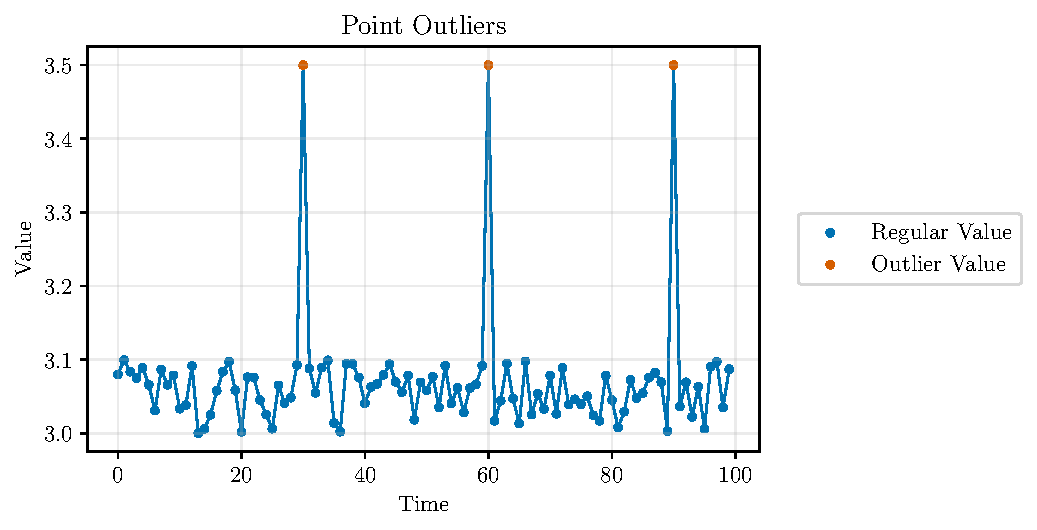
\includegraphics{./plots/pdfs/point_outliers.pdf}
  \caption{Examples of three point outliers}
  \label{figure:point-outliers}
\end{figure}

\subsubsection{Subsequence outliers}
Subsequence outliers are multiple consecutive datapoints that strongly vary from the usual trend of the datapoints. \cite{blazquez-garciaReviewOutlierAnomaly2020} In \autoref{figure:subsequence-outliers} examples of subsequence outliers are shown.
\newline\newline
\begin{figure}[h]
  \centering
  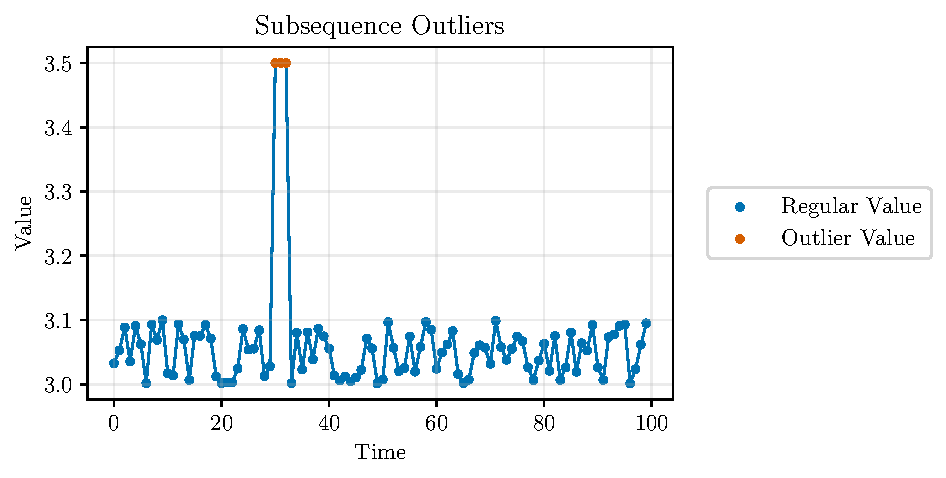
\includegraphics{./plots/pdfs/subsequence_outliers.pdf}
  \caption{Examples of three subsequence outliers}
  \label{figure:subsequence-outliers}
\end{figure}
Furthermore outliers can be divided into local and global outliers. 
\subsubsection{Local Outliers}
A local outlier has a greater variance to its direct neighbouring datapoints (previous and next one) \cite{blazquez-garciaReviewOutlierAnomaly2020} In \autoref{figure:local-point-outliers} and \autoref{figure:local-subsequence-outliers} examples of local outliers are shown. The first two outliers in \autoref{figure:local-point-outliers} have a great variance towards it direct neighbours, however not to the values from Time 60 onwards.
\begin{figure}[H]
  \centering
  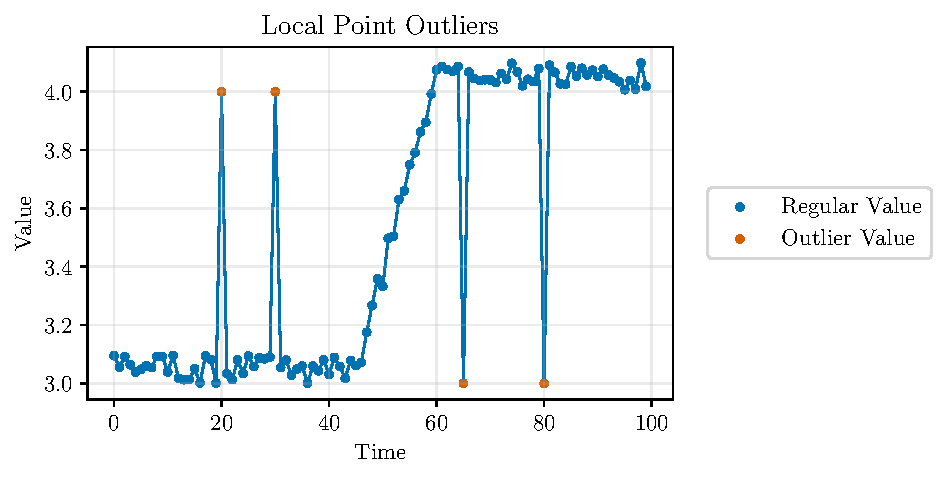
\includegraphics{./plots/pdfs/local_point_outliers.pdf}
  \caption{Examples of four local point outliers}
  \label{figure:local-point-outliers}
\end{figure}
\begin{figure}[H]
  \centering
  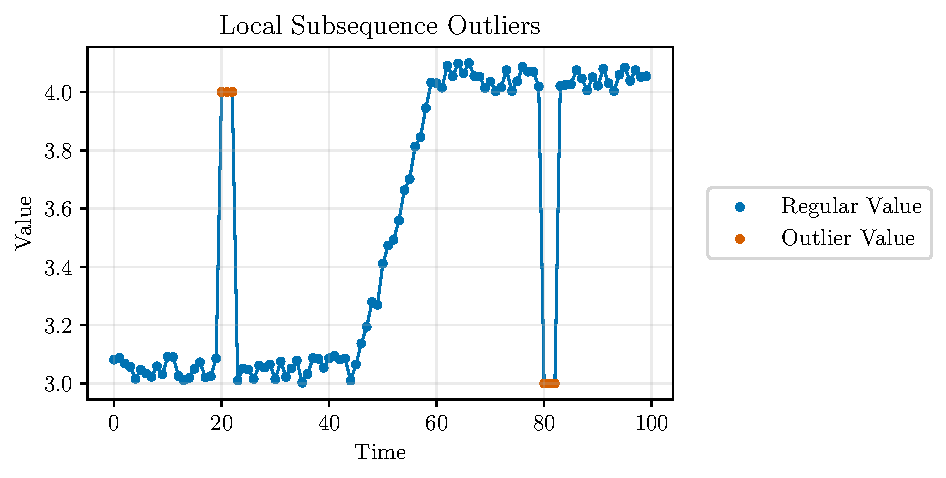
\includegraphics{./plots/pdfs/local_subsequence_outliers.pdf}
  \caption{Examples of six local subsequence outliers}
  \label{figure:local-subsequence-outliers}
\end{figure}
\subsubsection{Global Outliers}
Whereas a global outlier varies more in regard to all datapoints. \autoref{figure:point-outliers}, \ref{figure:subsequence-outliers} and \ref{figure:global-point-outliers} show picture examples of global outliers.
\cite{blazquez-garciaReviewOutlierAnomaly2020}
\begin{figure}[H]
  \centering
  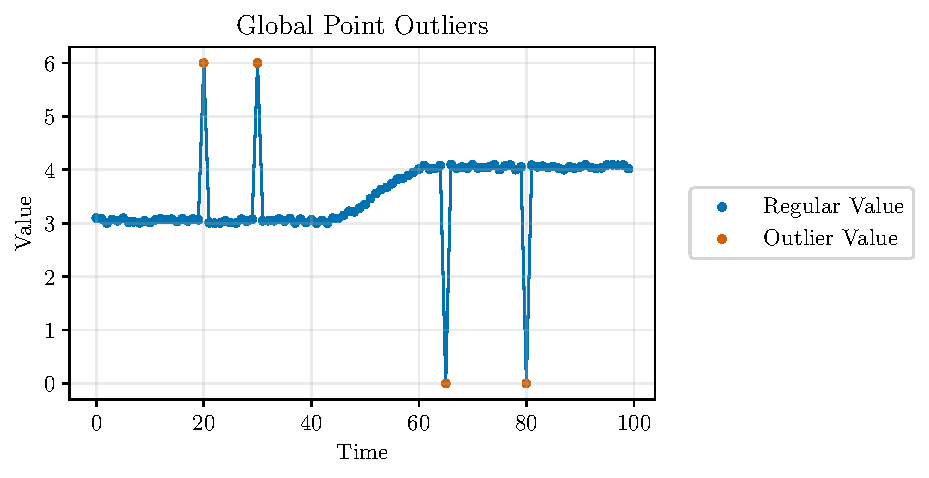
\includegraphics{./plots/pdfs/global_point_outliers.pdf}
  \caption{Examples of four global point outliers}
  \label{figure:global-point-outliers}
\end{figure}

\section{Outlier Detection Approaches}\label{section:outlier-detection-approaches}
Outlier detection methods can be divided into the following groups
\subsubsection{Statistical}
For statistical outlier detection, historical data is taken to develop a model that pictures the expected behavior of the data. An example of a statistical outlier detection is the threshold based method described in \autoref{section:threshold-based-outlier-detection} \cite{cookAnomalyDetectionIoT2020, giannoniAnomalyDetectionModels2018}

\subsubsection{Distance based}
For this approach a distance metric needs to be defined, (e.g. Euclidean distance). Then each datapoint is compared to the data preceding it. The greater the distance between the current and previous datapoints the greater the probability of an anomaly. \cite{cookAnomalyDetectionIoT2020, giannoniAnomalyDetectionModels2018, chandolaAnomalyDetectionSurvey2009}

\subsubsection{Clustering}
Clustering also requires a set of historical data in order to train the clustering model. Usually the data is clustered into two clusters: normal data and anomalous data. Depending on the distance of a new datapoint to the "normal" and the "anomalous" cluster it is classified.
\cite{cookAnomalyDetectionIoT2020, giannoniAnomalyDetectionModels2018, chandolaAnomalyDetectionSurvey2009}
\subsubsection{Predictive}
In this approach a prediction model needs to be developed, based on previous data. The prediction of this model is then compared with the actual datapoint (new data, which was not used in training the model). If the actual datapoint differs too much from the prediction it is labelled as an anomaly. \cite{cookAnomalyDetectionIoT2020, giannoniAnomalyDetectionModels2018}


\subsubsection{Ensemble}
as the word ensemble suggests, this is a collection of outlier detection methods that use a specific vote mechanism to determine whether a datapoint is faulty or normal. For example using the majority vote system and a statistical, distance based and predictive method to detect outliers. If at least two methods flag a datapoint as an outlier the ensemble reports it as an outlier as well. If only one method reports it as an outlier the ensemble does not flag it as an anomaly.
\cite{cookAnomalyDetectionIoT2020}

\section{Threshold based Outlier Detection}\label{section:threshold-based-outlier-detection}
Threshold based detection methods are able to identify outliers based on a given threshold $\tau$. These Methods can be described with the following formula
$$
  |x_t - \hat{x}_t | > \tau \text{ \cite{blazquez-garciaReviewOutlierAnomaly2020}}
$$
Where $x_t$ is the actual value and $\hat{x}_t$ is the expected value and $\tau$ is a given threshold.\\
Methods to calculate $\hat{x}_t$ will be described in the following sections. Furthermore $\hat{x}_t$ can be calculated using the entire data series or with subsets (of equal length) of the entire data series. This means $\hat{x}_t$ can be either calculated for the whole data series or for just a segment.\\
Depending on the sensitivity wanted for outlier detection an appropriate $\tau$ needs to be chosen. The greater $\tau$ is the fewer outliers will be detected. The smaller $\tau$ is the more outliers will be identified.  \cite{blazquez-garciaReviewOutlierAnomaly2020}

\subsubsection{Mean}
$$
  \text{mean} = \overline{x} = \frac{1}{n} \sum^n_{t=0}x_t
$$
Where $n$ is the total number of samples. Using the mean as an expected value is not robust to outliers, because the median is not as robust as the mean in hindsight to outliers. To calculate the mean all datapoints of a series must be summed up and then divided by the number of datapoints.
\subsubsection{Median}
If $n$ is odd:
$$
  median(x) = x_{(n+1)/2}
$$
If $n$ is even:
$$
  median(x) = \frac{x_{n/2} + x_{(n+1)/2}}{2}
$$
Where $x$ is a dataset of $n$ elements ordered from smallest to largest\\
($x_1 \leq x_2 \leq x_3 \leq \ldots \leq x_{n-2} \leq x_{n-1} \leq x_n$)
\cite{blazquez-garciaReviewOutlierAnomaly2020}
To calculate the median all values must be sorted from smallest to largest. If the number of datapoints is odd then the most center datapoint is the Median (e.g. if the series consist of 7 values the third value is the median). If the number of datapoints is even then the median is the mean of the two datapoints in the center.
\subsubsection{Median Absolute Deviation (\ac{MAD})}
The Median Absolute Deviation 
$$
  MAD = median(|x_t - median(x)|)
$$
$MAD$ is a more robust (regarding outliers) way to calculate the deviation of a dataset. To calculate the $MAD$ firstly the median of the dataset must be calculated. Then the absolute difference between $x_t$ and the median of the dataset is calculated. The Median of all differences results in the $MAD$
\cite{leysDetectingOutliersNot2013, mehrangOutlierDetectionWeight2015}

\section{Outlier Detection using the z-score}


\section{Other Variants of Outlier Detection Methods}
Provide a deeper insight in other outlier detection approaches. E.g. Clustering / predictive or distance based.
\todo{Research other outlier detection methods}
\chapter{Outlier Detection based on Water Level Data}
FloodAlert (or ``Pegelalarm'' in German) is a service that provides water levels from about 30,000 measurement stations. It provides notifications to registered individuals, when a certain water level threshold is reached. Thus warning people about possible floods in their area. \cite{strassmayrFloodAlertWaterLevels}


Unfortunately sometimes an incorrect water level is reported by the sensors, which are not maintained by the team of FloodAlert. FloodAlert just fetches the data from different maintainers of sensors. To reduce the frequency of false alarms, outliers should be identified and flagged. The theoretical parts of the previous sections are applied and tested on real-word data.
% Create a connection between the theoretical descriptions of outlier detections to a real world use case. Data from \url{https://pegelalarm.at/}
% \todo{write}
\section{What is the Goal?}
The ideal goal of FloodAlert would be to have a general model, that works on a variety of rivers. The model should be able to predict the probability of being an outlier for each water level value, without knowing future values. Thereby making it possible to classify incoming datapoints in real time, without needing future datapoints to make a prediction. Furthermore it would be ideal if the outlier detection method is able to adjust its parameters automatically for each river / water level measurement location. Because different rivers have different fluctuations in water level. Therefore each water level measurement station needs individual parameters. For example one river regularly has an increase and decrease of 10 centimeters whereas for another river 10 cm of water level variance from one datapoint to the next is definitely an outlier.
\newline
\newline
Another approach would be to also take future values into consideration when predicting the probability of a value being an outlier. This method is probably easier and likely leads to better results. However a method which does not take future values into consideration would be more useful for FloodAlert, since the values could be classified immediately.

% Describe the goal to archive: \newline
% \todo{change this}
% \begin{itshape}
%     ``
%     \begin{enumerate}
%         \item We are looking for an algorithm that detects outliers using only historical values. This would allow us to assign a probability to the last measured water level of a station, which would indicate how likely it is to be an outlier. We would then not store outliers in our system at all or classify them as outliers from the beginning.
%         \item For us also an algorithm would be helpful, which assigns an outlier probability to each arbitrary measured value X of a time series. This algorithm would not only have access to the measured values before it, but also to those after it. This would allow us to detect outliers for all the time series data that we already have in the system and, for example, delete them.

%     \end{enumerate}
%     Point 2 is probably easier to implement than point 1, so an algorithm 1 would be more helpful for us.
%     Also important would be that the algorithm adjusts its (hyper)parameters accordingly based on the historical data. This means that a level at which there are often strong fluctuations, an outlier must already be quite outlier so that it is considered as an outlier.
%     ''
% \end{itshape}

\section{How to retrieve the Data (Description of the API)}
% Short overview on how to use the API to retrieve data? Python project to retrieve data: \url{https://github.com/SOBOS-GmbH/pegelalarm_public_pas_doc}
To make the access to the API easier SOBOS GmbH developed a Python wrapper which returns the requested data as a Pandas dataframe.\cite{PandasDocumentationPandas} The code for the Python wrapper is available on GitHub\cite{GitHub}: \url{https://github.com/SOBOS-GmbH/pegelalarm_public_pas_doc} \cite{strassmayrPegelalarmAPIWrapper2022}

In order to request data, an API key needs to be requested using credentials. To request the API key a POST request needs to be sent to this endpoint \url{https://api.pegelalarm.at/api/login}, where the request body contains the users' credentials as shown in \autoref{listing:api-key-request-body}. 
\begin{listing}
\begin{minted}[linenos]{json}
{
    "username": "myUsername",
    "password": "myPassword"
}
\end{minted}
\caption{Request body to get API key}
\label{listing:api-key-request-body}
\end{listing}
To generate the actual API key the key from the response needs to be hashed using the \ac{HMAC} Algorithm. This is done using Python's built in ``hmac'' module. \cite{HmacKeyedHashingMessage}. Afterwards the \ac{HMAC} is byte64 encoded, so it can be sent in the ``X-AUTH-TOKEN'' header field.

To get the unique identifier for a specific measurement station the list endpoint can be used. Which accepts three optional query parameters (qStationName - station name, qWater - water name and commonid - the unique identifier of a station) and returns a list of matching stations with metadata like coordinates, country or last water level. E.g. to retrieve the identifier of the Danube station located in Linz the URL is the following: \url{https://api.pegelalarm.at/api/station/1.1/list?qStationName=Linz&qWater=Donau}. Keep in mind in order to retrieve any data the header value ``X-AUTH-TOKEN'' must be set. An example response of this request is shown in \autoref{listing:response-list-endpoint}. Where the unique identifier is the ``commonid'' in line 9.
\begin{listing}
\begin{minted}[linenos]{json}
{
    "status": {
        "code": 200
    },
    "payload": {
        "stations": [
            {
                "name": "Donau / Linz / at",
                "commonid": "207068-at",
                "country": "Österreich",
                "stationName": "Linz",
                "water": "Donau",
                "region": "Oberösterreich",
                "latitude": 48.306915712282,
                "longitude": 14.284689597541,
                "positionKm": 2135.17,
                "altitudeM": 247.74,
                "defaultWarnValueCm": 550.0,
                "defaultAlarmValueCm": 630.0,
                "data": [
                    {
                        "type": "height in cm",
                        "value": 358.0,
                        "requestDate": "19.04.2022T14:59:51+0200",
                        "sourceDate": "19.04.2022T14:45:00+0200"
                    }
                ],
                "trend": 10,
                "situation": 10,
                "visibility": "PUBLIC",
                "stationType": "surfacewater"
            }
        ]
    }
}
\end{minted}
\caption{Example response of the list endpoint}
\label{listing:response-list-endpoint}
\end{listing}

To retrieve historical data, the history endpoint can be used. The request URL has the following structure: \url{https://api.pegelalarm.at/api/station/1.1/<unit>/<commonid>/history?<parameters>}. The unit can either be ``height'' or ``flow''. For this thesis only height data was used. The following parameters can be set:
\begin{itemize}
    \item \textbf{loadStartDate}: The start timestamp of the queried data.
    \item \textbf{loadEndDate}: The end timestamp of the queried data.
    \item \textbf{granularity}: The granularity of the response. 
\end{itemize}
Possible values for the granularity are: ``raw'' (for the last 3 months of data), ``hour'', ``day'', ``month'', ``year'' or ``era'' (era returns one value for a given time)
When requesting aggregated data (anything other than ``raw''), the maximum value of the timespan is used. The timestamps are in the following format: ``<DD>.<MM>.<YYYY>T<HH>:<MM>:<SS><+-UTCOFFSET>'', where the `+' is URL encoded to ``\%2B''. E.g.: ``31.03.2022T13:35:40\%2B0200''. If no parameters are provided the API returns the last few datapoints.

An example request would be: \url{https://api.pegelalarm.at/api/station/1.1/height/207068-at/history?loadStartDate=01.03.2022T13:35:40%2B0200&loadEndDate=01.03.2022T18:00:00%2B0200&granularity=hour} The result of this request is shown in \autoref{listing:water-level-data-response}.

\begin{listing}
\begin{minted}[linenos]{json}
{
    "status": {
        "code": 200
    },
    "payload": {
        "history": [
            {
                "value": 360.0,
                "sourceDate": "01.03.2022T13:00:00+0100"
            },
            {
                "value": 360.0,
                "sourceDate": "01.03.2022T14:00:00+0100"
            },
            {
                "value": 359.0,
                "sourceDate": "01.03.2022T15:00:00+0100"
            },
            {
                "value": 361.0,
                "sourceDate": "01.03.2022T16:00:00+0100"
            },
            {
                "value": 362.0,
                "sourceDate": "01.03.2022T17:00:00+0100"
            }
        ]
    }
}
\end{minted}
\caption{Example response of historical water level data for one station}
\label{listing:water-level-data-response}
\end{listing}

\section{Overview of the Data}
To test and tune the outlier detection methods the entire history of data was used. The granularity of the data usually is hourly up to the last three months of data. There are a few exceptions, where the granularity is not hourly, because either one or a few datapoints are missing. For the last three months the granularity is ``raw'', which is different for each station. Additionally the base (where the sensor reports water level equals zero) also differs per station. Some station have an arbitrary zero level whereas some stations have the sea level as a base. Thus the water level does not actually reflect the actual height, or depth, of the water. Instead it represents the relative water level to a specific height.
\par
The following water level measurement stations were used to test the outlier detection methods.
\change{Check and maybe remove automatic hyphenation}
% \begin{itemize}
%     % \item List of station addresses \todo{add final stations} 
%     \todo{add location description to station list}
%     \item Station Aghacashlaun, Aghacashlaun (36022-ie)
%     \item Station 2386-ch
%     \item Station 2720050000-de
%     \item Station 42960105-de
%     \item Station 39003-ie
% \end{itemize}
\subsubsection{Station Aghacashlaun, Aghacashlaun (36022-ie)}
This station, on the river Aghacashlaun and in the area of Aghacashlaun, is located in northern Ireland. The coordinates of this station are: 54.03647, -7.94672 (\ac{Lat}, \ac{Long}). \cite{StationAghacashlaunAghacashlaun}

\subsubsection{Station Murg, Frauenfeld (2386-ch)}
The station, on the river Murg and in the area of Frauenfeld, is located in northern Switzerland. The coordinates of this station are: 47.56852, 8.89432 (\ac{Lat}, \ac{Long}). \cite{StationMurgFrauenfeld}

\subsubsection{Station Sieg, Betzdorf (2720050000-de)}
The station, on the river Sieg and in the area of Betzdorf, is located in western Germany. The coordinates of this station are: 50.79332, 7.86390 (\ac{Lat}, \ac{Long}). \cite{StationSiegBetzdorf}

\subsubsection{Station Losse, Helsa (42960105-de)}
The station, on the river Losse and in the area of Helsa, is located in central Germany . The coordinates of this station are: 51.25574, 9.68537 (\ac{Lat}, \ac{Long}). \cite{StationLosseHelsa}

\subsubsection{Station Crana, Tullyarvan (39003-ie)}
The station, on the river Crana and in the area of Tullyarvan, is located in northern Ireland. The coordinates of this station are: 55.14356, -7.45239 (\ac{Lat}, \ac{Long}). \cite{StationCranaTullyarvan}

\section{Manually detect outliers for a subset of data}
% \todo{add examples of outliers in the data}
% \todo{Describe how the outliers are stored?}
% Show cases of outliers in the data and manually classify them. (Also define a way/data structure to classify outliers for time series data) \todo{Remove this}
In order to speed up the manual labeling of outliers a program was written. The program is a Plotly Dash \cite{DashDocumentationUser} \change{Which reference to add? Website, Documentation or GitHub?} web application which displays the water level data as a scatter chart. 
By clicking the datapoints in the chart the user is able to toggle the datapoint as an outlier or back to a regular value. 
In Listing \ref{listing:manual-outlier-selection} the source code of the Dash application is shown. 
In \autoref{figure:manual-outlier-selection} the Website of the Python app is shown, the red dots between 25 and October 28 are already classified outliers. Below the chart a rangeslider is located, to move the zoomed in view horizontally. 
The refresh button on the left side refreshes the graph, thus updating the color and label of previously selected outliers. Furthermore it saves the data to a parquet file.
The upper and lower limit of the y-axis also gets updated, when pressing the refresh button. 
The limits are automatically set to the lowest and highest regular value. 
This was implemented, because some datasets had outliers with a huge difference towards the regular data. 
Without the automatic scaling of the y-axis, detecting other outliers with a smaller difference was not possible.
% \begin{center}
%     \makebox[\textwidth]{\includegraphics[width=\paperwidth]{...}}
%   \end{center}
\begin{figure}[H]
    \centering
    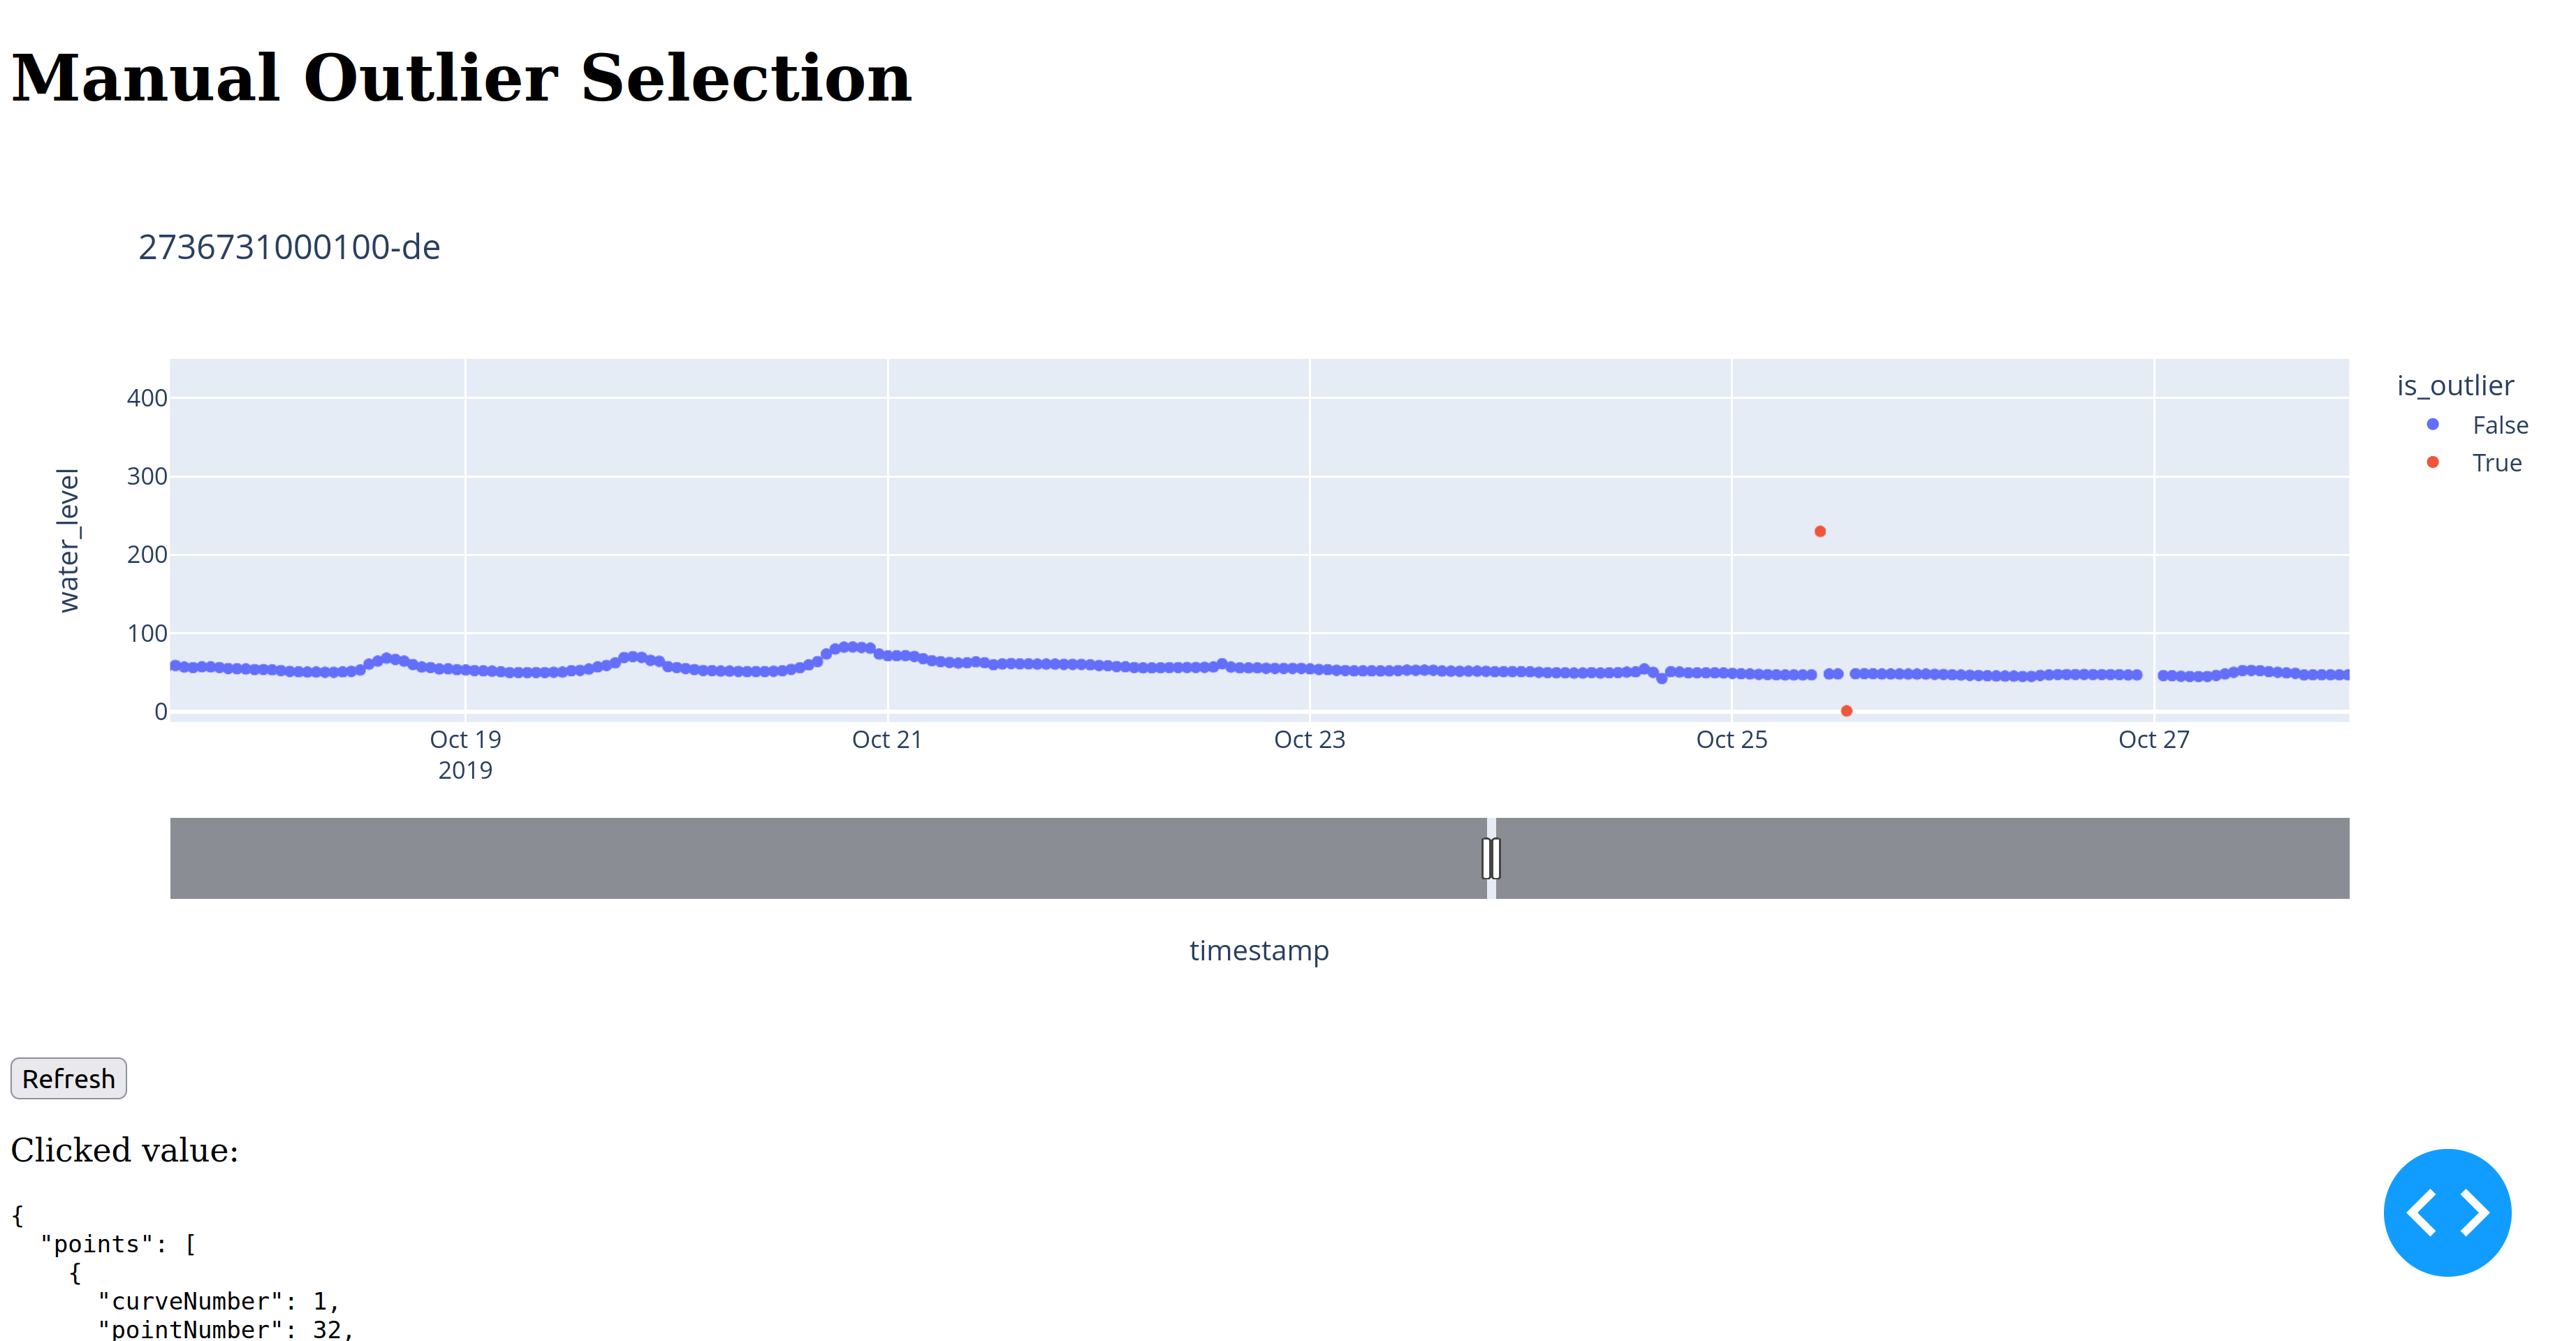
\includegraphics[width=\textwidth]{./pics/manual-outlier-selection.png}
    \caption{Dash Webapp to classify outliers}
    \label{figure:manual-outlier-selection}
\end{figure}

% https://tex.stackexchange.com/questions/368864/pagebreak-for-minted-in-figure
% \begin{listing}
% \begin{minted}[frame=single]{python}
% print('hw')
% \end{minted}
% \caption{Code example with simple formatting}
% \label{code:manual-outlier-selection}
% \end{listing}

\subsubsection{Manual Outlier Detection Webapp using Dash}
\inputminted[linenos]{python}{./code/manual_outlier_detection.py}
\captionof{listing}{Manual Outlier Detection Webapp using Dash\label{listing:manual-outlier-selection}}
\todo{add comments to code}

\section{Explorative Data Analysis}
\todo{add another station}
\todo{add line chart over whole time with 1-2 zooms}
\subsection{Aghacashlaun Station}
% Similar to overview of the data
% \begin{figure}[H]
%     \centering
%     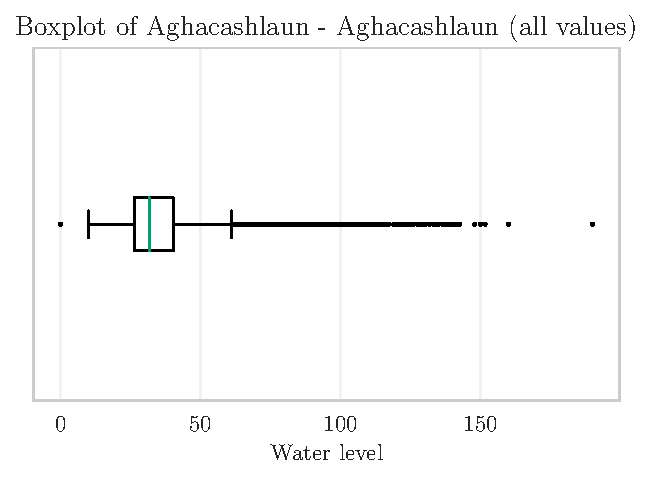
\includegraphics{./plots/pdfs/36022-ie/boxplot_36022-ie_all.pdf}
%     \caption{Boxplot of Aghacashlaun - Aghacashlaun containing all values}
%     \label{figure:boxplot-36022-ie-all}
% \end{figure}
% \begin{figure}[H]
%     \centering
%     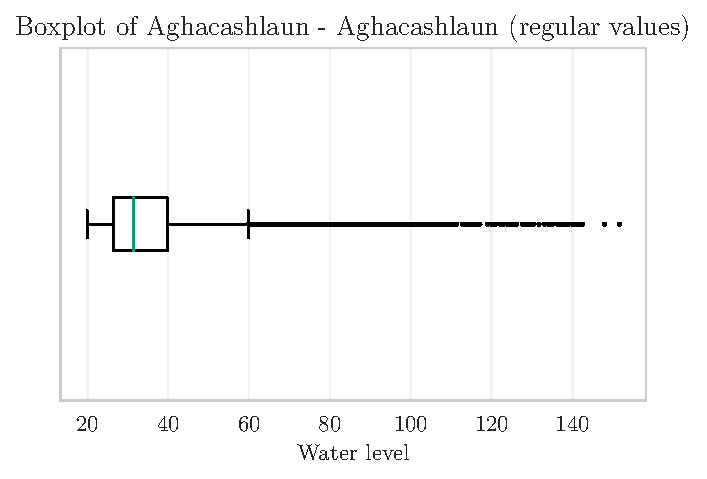
\includegraphics{./plots/pdfs/36022-ie/boxplot_36022-ie_regular.pdf}
%     \caption{Boxplot of Aghacashlaun - Aghacashlaun containing regular values}
%     \label{figure:boxplot-36022-ie-regular}
% \end{figure}

% \begin{figure}[H]
%     \centering
%     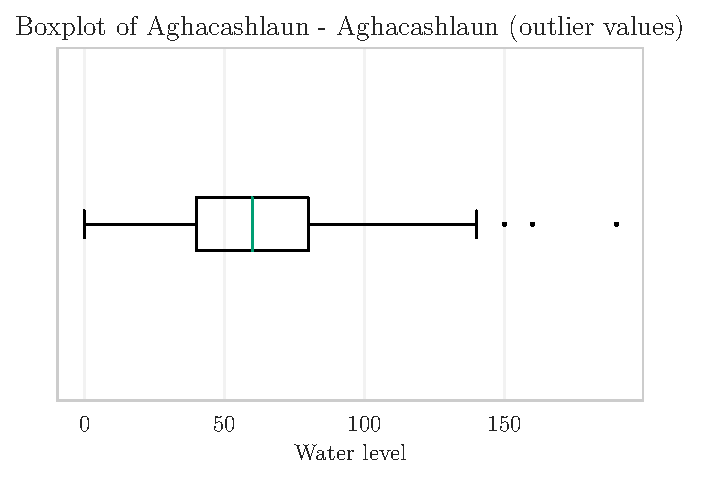
\includegraphics{./plots/pdfs/36022-ie/boxplot_36022-ie_outlier.pdf}
%     \caption{Boxplot of Aghacashlaun - Aghacashlaun containing outlier values}
%     \label{figure:boxplot-36022-ie-outlier}
% \end{figure}
\todo{change formatting of tables}
\begin{table}
\centering
\begin{tabular}{lrrr}
\toprule
{} &   water\_level &  water\_level\_diff &     timedelta \\
\midrule
count &  27189.000000 &      27188.000000 &  27188.000000 \\
mean  &     36.009754 &         -0.000077 &      0.809990 \\
std   &     14.716286 &          7.220175 &      1.256409 \\
min   &      0.000000 &       -107.500000 &      0.000000 \\
25\%   &     26.400000 &         -0.300000 &      1.000000 \\
50\%   &     31.700000 &         -0.100000 &      1.000000 \\
75\%   &     40.300000 &          0.000000 &      1.000000 \\
max   &    190.000000 &         94.800000 &    178.000000 \\
\bottomrule
\end{tabular}
\caption{Seven number summary of Aghacashlaun - Aghacashlaun (all values)}
\label{table:36022-ie-7-number-summary-all}
\end{table}

\begin{table}[htp]
\centering
\begin{tabular}{lrrr}
\toprule
{} &   water\_level &  water\_level\_diff &     timedelta \\
\midrule
count &  26544.000000 &      26543.000000 &  26543.000000 \\
mean  &     35.381205 &         -0.411276 &      0.808311 \\
std   &     13.763332 &          5.165770 &      1.268532 \\
min   &     20.000000 &       -107.500000 &      0.000000 \\
25\%   &     26.400000 &         -0.300000 &      1.000000 \\
50\%   &     31.400000 &         -0.100000 &      1.000000 \\
75\%   &     39.800000 &          0.000000 &      1.000000 \\
max   &    151.600000 &         51.900000 &    178.000000 \\
\bottomrule
\end{tabular}
\caption{Seven number summary of Aghacashlaun - Aghacashlaun (regular values)}
\label{table:36022-ie-7-number-summary-regular}
\end{table}

\begin{table}[htp]
\centering
\caption{Seven number summary of Aghacashlaun - Aghacashlaun (outlier values)}
\label{table:36022-ie-7-number-summary-outlier}
\begin{tabular}{lrrr}
\toprule
{} &  water\_level &  water\_level\_diff &   timedelta \\
\midrule
count &   645.000000 &        645.000000 &  645.000000 \\
mean  &    61.876744 &         16.921550 &    0.879070 \\
std   &    25.476859 &         28.411003 &    0.560844 \\
min   &     0.000000 &        -90.000000 &    0.000000 \\
25\%   &    40.000000 &        -10.000000 &    1.000000 \\
50\%   &    60.000000 &         12.500000 &    1.000000 \\
75\%   &    80.000000 &         39.400000 &    1.000000 \\
max   &   190.000000 &         94.800000 &    9.000000 \\
\bottomrule
\end{tabular}
\end{table}


\begin{figure}[htp]
    \centering
    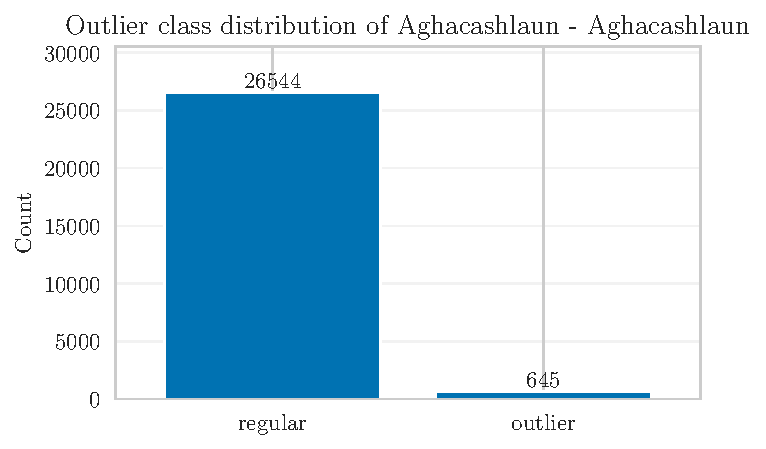
\includegraphics{./plots/pdfs/36022-ie/outlier_class_distribution_36022-ie.pdf}
    \caption{Class distribution of Aghacashlaun - Aghacashlaun}
    \label{figure:class-distribution-36022-ie}
\end{figure}

\begin{figure}[htp]
    \centering
    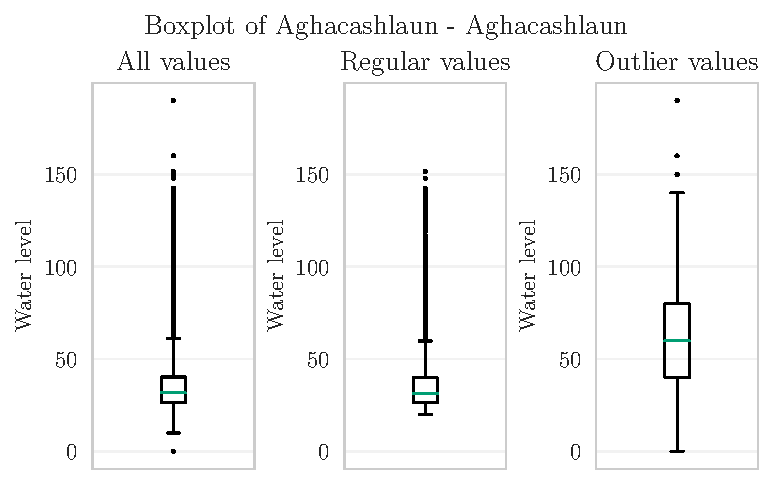
\includegraphics{./plots/pdfs/36022-ie/boxplot_36022-ie.pdf}
    \caption{Boxplot of Aghacashlaun - Aghacashlaun}
    \label{figure:boxplot-36022-ie}
\end{figure}

\begin{figure}[htp]
    \centering 
    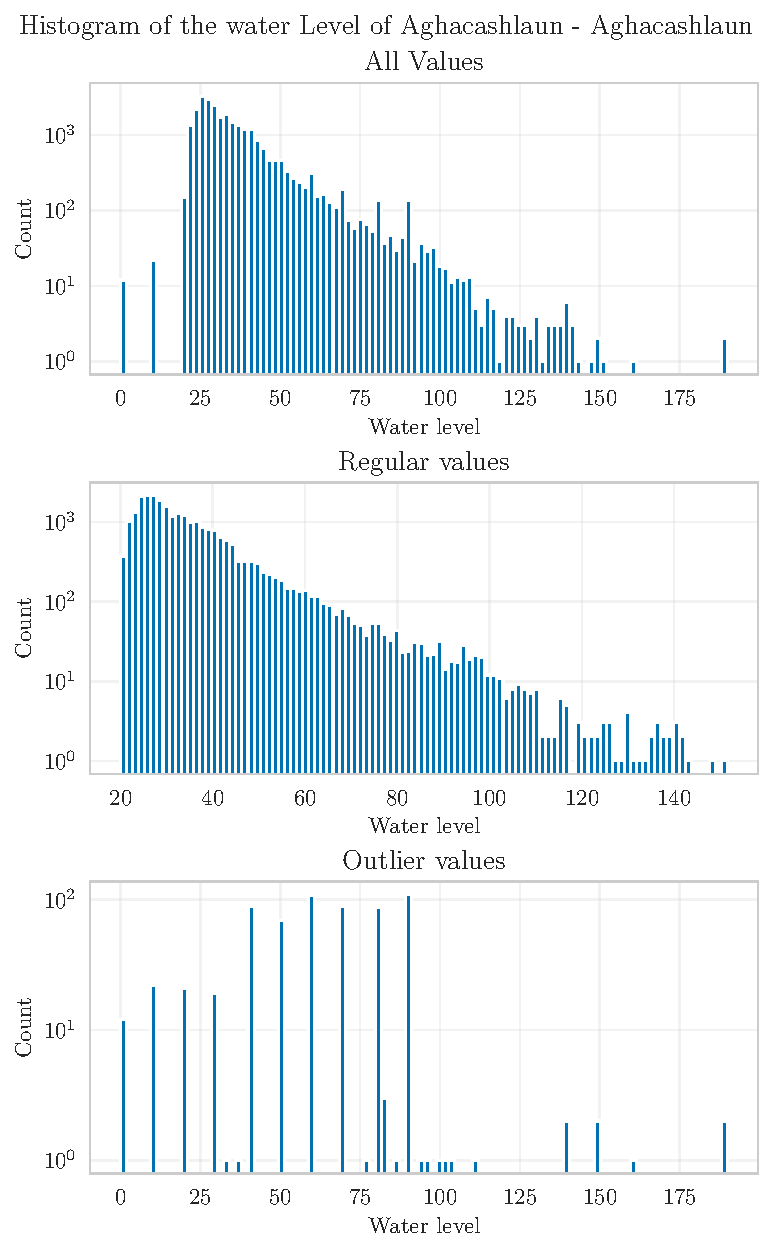
\includegraphics{./plots/pdfs/36022-ie/water_level_histogram_36022-ie.pdf}
    \caption{Histogram of the water level of Aghacashlaun - Aghacashlaun}
    \label{figure:water-level-histogram-36022-ie}
\end{figure}

\begin{figure}[htp]
    \centering
    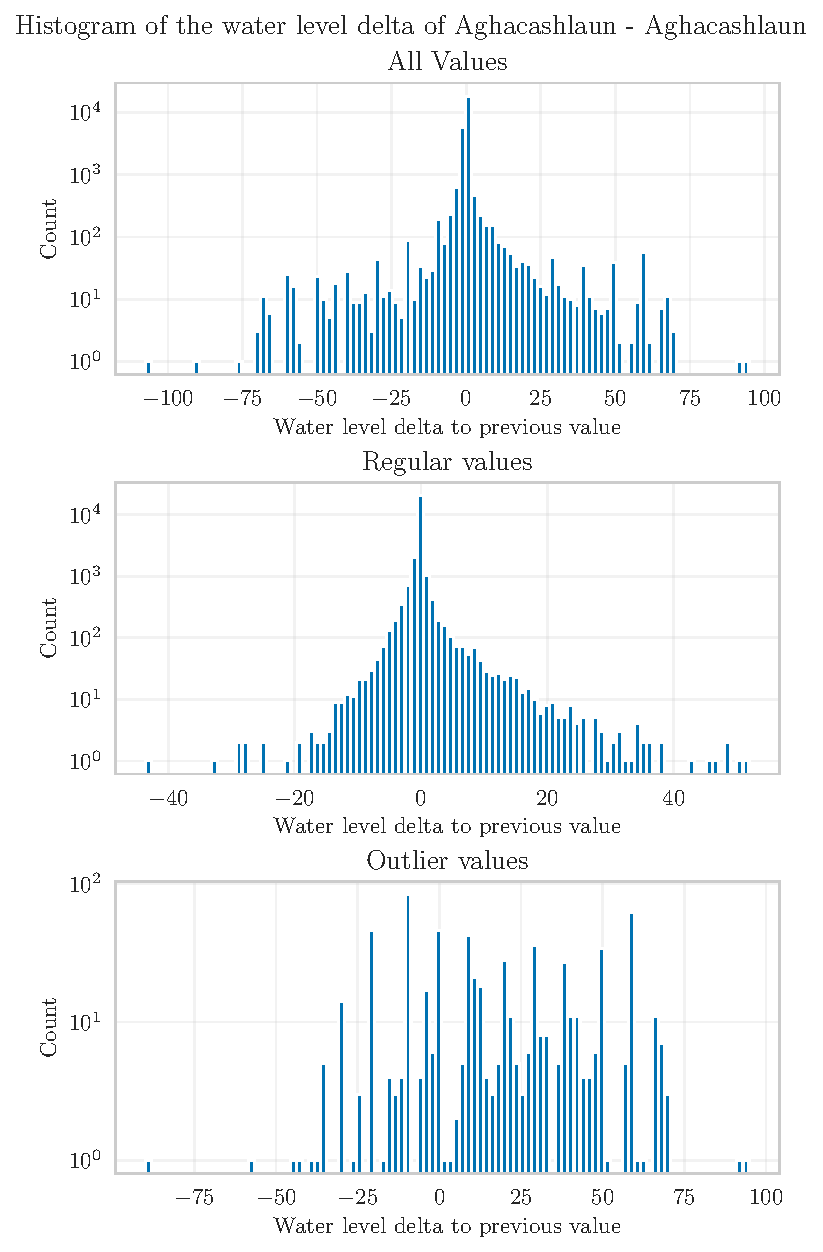
\includegraphics{./plots/pdfs/36022-ie/water_level_delta_histogram_36022-ie.pdf}
    \caption{Histogram of the water level delta of Aghacashlaun - Aghacashlaun}
    \label{figure:water-level-delta-histogram-36022-ie}
\end{figure}

\begin{figure}[htp]
    \centering
    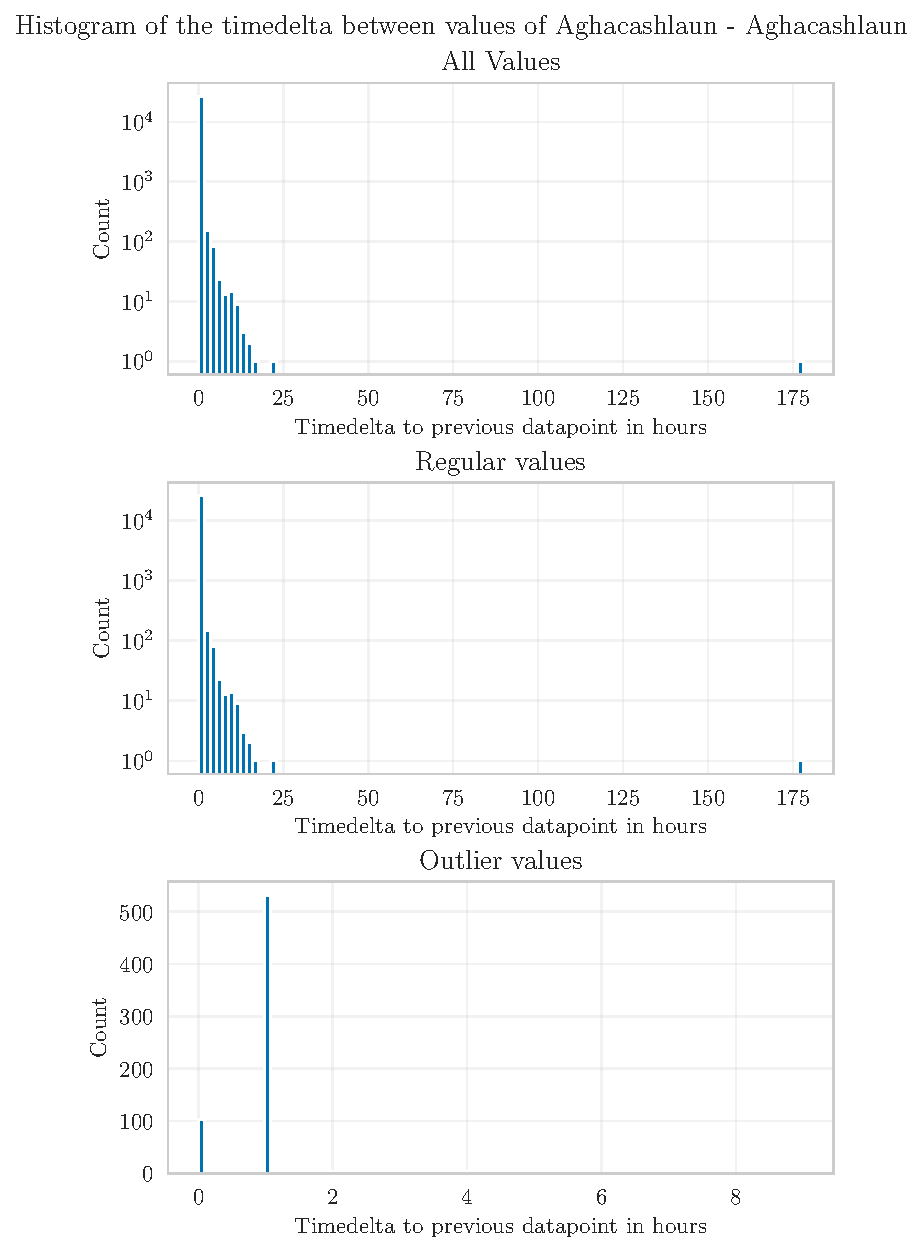
\includegraphics{./plots/pdfs/36022-ie/time_delta_histogram_36022-ie.pdf}
    \caption{Histogram of the time delta (in hours) of Aghacashlaun - Aghacashlaun}
    \label{figure:time-delta-histogram-36022-ie}
\end{figure}
\par
Code: \cite{zelenayOutlierDetectionWater2022}
\todo{add descriptions to tables and figures}

\section{Outlier Detection performance Metrics}
\subsection{Confusion Matrix}
To compare the performance of two classification methods a confusion matrix, shown in \autoref{table:confusion-matrix}, can be used to provide an overview. A confusion matrix consists of the following elements (explained on the basis of outlier detection):
\begin{itemize}
    \item \ac{TP}: actual class: outlier, predicted class: outlier
    \item \ac{FN}: actual class: outlier, predicted class: regular
    \item \ac{TN}: actual class: regular, predicted class: regular
    \item \ac{FP}: actual class: regular, predicted class: outlier
\end{itemize}
\begin{table}[ht]
    \begin{tabular}{llll}
     &  & \multicolumn{2}{l}{Predicted label} \\ \cline{3-4} 
     & \multicolumn{1}{l|}{} & \multicolumn{1}{l|}{\ac{P}} & \multicolumn{1}{l|}{\ac{N}} \\ \cline{2-4} 
    \multicolumn{1}{l|}{} & \multicolumn{1}{l|}{Positive} & \multicolumn{1}{l|}{\cellcolor[HTML]{9AFF99}True positive} & \multicolumn{1}{l|}{\cellcolor[HTML]{FFCCC9}False negative} \\ \cline{2-4} 
    \multicolumn{1}{l|}{\multirow{-2}{*}{True/ actual label}} & \multicolumn{1}{l|}{Negative} & \multicolumn{1}{l|}{\cellcolor[HTML]{FFCCC9}False positive} & \multicolumn{1}{l|}{\cellcolor[HTML]{9AFF99}True negative} \\ \cline{2-4} 
\end{tabular}
\caption{Example of binary confusion matrix}
\label{table:confusion-matrix}
\end{table}
% ausser publikation welche nur cm behandelt
% \todo{add reference? \url{https://en.wikipedia.org/w/index.php?title=Confusion_matrix&oldid=1058352752}}
The green cells represent the correctly classified values (\ac{TP} \& \ac{TN}) and the red cells represent the incorrectly classified values (\ac{FN} \& \ac{FP}). The confusion matrix is the basis of many more performance metrics.
\subsection{Accuracy}
To make the comparison easier, the confusion matrix can be aggregated into one single value as a metric. There are numerous ways how this single metric can be calculated. One of the Most common and basic methods is the Accuracy:
\begin{equation}
    Accuracy = \frac{Number\,of\,correct\,predictions}{Total\,number\,of\,predictions} = \frac{TP + TN}{TP + FN + TP + FP} = \frac{TP + TN}{P + N}
\end{equation}
The accuracy provides information what percentage of values are correctly classified. However if the classes are not equally distributed, the accuracy is a bad metric. This is especially true for heavily imbalanced classes. For example if the dataset has $1\,000\,000$ positive values and $10$ negative, when optimizing for a high accuracy it can happen that the classifier predicts every value as positive and still achieves a very high accuracy:
\begin{equation}
    Accuracy = \frac{1\,000\,000 + 0}{1\,000\,000 + 10} = 0.99999
\end{equation}
Thus for measuring the performance of outliers, the accuracy is not a suitable metric.

\subsection{Precision and Recall}
\autoref{figure:precision-vs-recall} shows a visual comparison between precision and recall. The precision provides information about what percentage of positive predictions were actually correct. Whereas the recall provides information about what percentage of all positive values were actually predicted as such. Precision and Recall are used to calculate the F-Score described in \autoref{subsection:f-score}.
\begin{figure}[H]
    \centering
    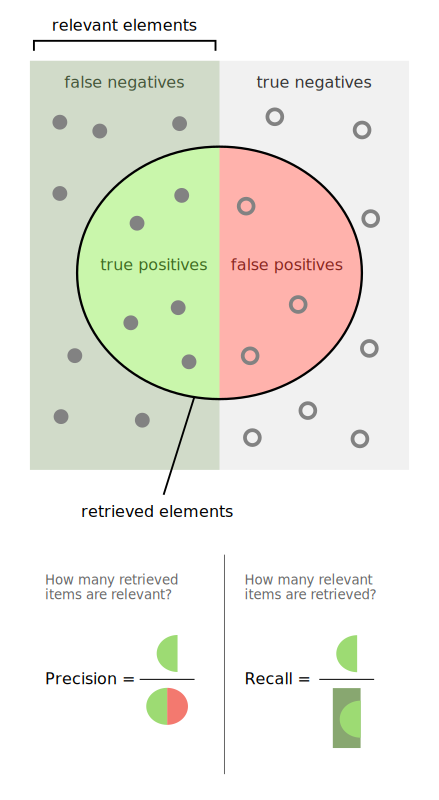
\includegraphics[width=\textwidth/2]{./pics/Precisionrecall.pdf}
    \caption{Precision vs Recall\cite{PrecisionRecall2022}}
    \label{figure:precision-vs-recall}
\end{figure}
% \todo{Correct reference of a image used 1:1? -> yes}
\subsubsection{Precision}
\begin{equation}
    Precision = \frac{TP}{TP + FP}
\end{equation}

\subsubsection{Recall}
\begin{equation}
    Recall = \frac{TP}{TP + FN}
\end{equation}

\subsection{F-score}
\label{subsection:f-score}
The $F_1-score$ is the harmonic mean of the precision and recall.
\begin{equation}
    F_1-score = \frac{2}{\frac{1}{Precision} + \frac{1}{Recall}} = \frac{2}{\frac{Precision + Recall}{Precision \cdot Recall}} = \frac{2 \cdot Precision \cdot Recall}{Precision + Recall}
\end{equation}
\cite{sasakiTruthFmeasure, chinchorMUC4EvaluationMetrics1992}

The $F_\beta-score$ is more sophisticated compared to the $F_1-score$ where an additional parameter ($\beta$) needs to be chosen, which is used to weight the precision.
\begin{equation}
    F_\beta-score = \frac{(\beta^2 + 1) \cdot Precision \cdot Recall}{\beta^2 \cdot Precsion + Recall}
\end{equation}
\cite{tahaMetricsEvaluating3D2015, chinchorMUC4EvaluationMetrics1992}
% This \cite{tahaMetricsEvaluating3D2015} references \cite{chinchorMUC4EvaluationMetrics1992}.\todo{chech whether this can also be included} often both are used.


The $F_1-score$ uses $1$ for $\beta$ so the precision and the recall are equally weighted.

% Why accuracy is bad in our case. Precision, Recall, F1 score

% Define a way to compare different outlier detection models / define performance metrics. E.g. number correct outliers, average confidence for the correct outliers, number of missed outliers,....

\section{Implementation of different Outlier Detection Approaches}

The input data structure for the different approaches is a pandas DataFrame.\cite{PandasDocumentationPandas} The structure of the DataFrame is equal for all measurement stations. It contains the following columns:
\begin{itemize}
    \item \verb|water_level|: the water level of the river in cm (datatype: float64)
    \item \verb|timestamp|: the date and time of the datapoint in UTC (datatype: datetime64[ns, UTC])
    \item \verb|is_outlier|: true or false depending if the value is an outlier (datatype: bool)
\end{itemize}
To test the performance of the models the column \verb|is_outlier| contains the ground truth, which was manually labeled. An example of the input data can be seen in \autoref{table:36022-ie-9head}.

\begin{table}[htp]
\footnotesize
\centering
\begin{tabular}{rll}
\toprule
 water\_level &                 timestamp &  is\_outlier \\
\midrule
        24.9 & 2019-06-30 15:00:00+00:00 &       False \\
        24.9 & 2019-06-30 16:00:00+00:00 &       False \\
        24.8 & 2019-06-30 17:00:00+00:00 &       False \\
        24.4 & 2019-06-30 18:00:00+00:00 &       False \\
        24.4 & 2019-06-30 19:00:00+00:00 &       False \\
        24.3 & 2019-06-30 20:00:00+00:00 &       False \\
        24.1 & 2019-06-30 21:00:00+00:00 &       False \\
        24.0 & 2019-06-30 22:00:00+00:00 &       False \\
        90.0 & 2019-06-30 23:00:00+00:00 &        True \\
\bottomrule
\end{tabular}
\caption{First 9 values of Aghacashlaun - Aghacashlaun}
\label{table:36022-ie-9head}
\end{table}

To speed up the process of calculating the result of the outlier detection method ($|x_t - \hat{x}_t|$, the z-score or the modified z-score) is all done in one step and in the second step the result of this calculation is compared against a range of thresholds.
\subsection{Mean Threshold}
Calculating $\hat{x}_t$ using the mean for a pandas DataFrame \cite{PandasDocumentationPandas} is quite straightforward and is shown in \autoref{listing:mean-outlier-calculation}. To reduce the amount of duplicate code, the imports are only included in \autoref{listing:mean-outlier-calculation}.
\begin{listing}
\begin{minted}[linenos]{python}
from typing import Union

import numpy as np
import pandas as pd


def mean_outlier_detection(input_df: pd.DataFrame,
                           window: Union[int, None],
                           center_window: bool):
    """
    Detects outliers in a dataframe using a (moving) average.
    :param input_df: the input dataframe where the values are stored
                     in the column water_level
    :param window: the size of the window, None if no window should
                   be used
    :param center_window: whether the window should be centered or not
    :return: a copy of the input dataframe where the column result
             should be compared to a threshold to detect outliers
    """
    od_df = input_df.copy()
    if window is None:
        od_df['x_hat'] = od_df['water_level'].mean()
    else:
        od_df['x_hat'] = \
            od_df['water_level'].rolling(window=window,
                                         center=center_window,
                                         min_periods=1).mean()
    od_df['result'] = np.abs(od_df['water_level'] - od_df['x_hat'])
    return od_df
\end{minted}
\caption{First step of classifying outliers using the mean}
\label{listing:mean-outlier-calculation}
\end{listing}

\subsection{Median Threshold}
The calculation of the median is quite similar to the mean. It is shown in \autoref{listing:median-outlier-calculation}.
\begin{listing}
\begin{minted}[linenos]{python}
def median_outlier_detection(input_df: pd.DataFrame,
                             window: Union[int, None],
                             center_window: bool):
    """
    Detects outliers in a dataframe using a (moving) average.
    :param input_df: the input dataframe where the values are stored
                     in the column water_level
    :param window: the size of the window, None if no window should
                   be used
    :param center_window: whether the window should be centered or not
    :return: a copy of the input dataframe where the column result
             should be compared to a threshold to detect outliers
    """
    od_df = input_df.copy()
    if window is None:
        od_df['x_hat'] = od_df['water_level'].median()
    else:
        od_df['x_hat'] = \
            od_df['water_level'].rolling(window=window,
                                         center=center_window,
                                         min_periods=1).median()
    od_df['result'] = np.abs(od_df['water_level'] - od_df['x_hat'])
    return od_df
\end{minted}
\caption{First step of classifying outliers using the median}
\label{listing:median-outlier-calculation}
\end{listing}

% \subsection{\ac{MAD} Threshold}
\subsection{MAD Threshold}
In \autoref{listing:mad-outlier-calculation} an example for an implementation for calculating the \ac{MAD} is provided.
\begin{listing}
\begin{minted}[linenos]{python}
def mad_outlier_detection(input_df: pd.DataFrame,
                          window: Union[int, None],
                          center_window: bool):
    """
    Detects outliers in a dataframe using a (moving) average.
    :param input_df: the input dataframe where the values are stored
                     in the column water_level
    :param window: the size of the window, None if no window should
                   be used
    :param center_window: whether the window should be centered or not
    :return: a copy of the input dataframe where the column result
             should be compared to a threshold to detect outliers
    """
    od_df = input_df.copy()
    if window is None:
        od_df['x_hat'] = np.median(
            np.abs(od_df['water_level'] - np.median(
                od_df['water_level'])))
    else:
        od_df['x_hat'] = \
            od_df['water_level'].rolling(window=window,
                                         center=center_window,
                                         min_periods=1).apply(
                lambda x: np.median(np.abs(x - np.median(x))))
    od_df['result'] = np.abs(od_df['water_level'] - od_df['x_hat'])
    return od_df
\end{minted}
\caption{First step of classifying outliers using the \ac{MAD}}
\label{listing:mad-outlier-calculation}
\end{listing}

\subsection{Z-Score}
\autoref{listing:z-score-outlier-calculation} shows how to calculate th z-score in Python.
\begin{listing}
\begin{minted}[linenos]{python}
def z_score_outlier_detection(input_df: pd.DataFrame,
                              window: Union[int, None],
                              center_window: bool):
    """
    Detects outliers in a dataframe using a (moving) average.
    :param input_df: the input dataframe where the values are stored
                     in the column water_level
    :param window: the size of the window, None if no window should
                   be used
    :param center_window: whether the window should be centered or not
    :return: a copy of the input dataframe where the column result
             should be compared to a threshold to detect outliers
    """
    od_df = input_df.copy()
    if window is None:
        od_df['mean'] = od_df['water_level'].mean()
        od_df['std'] = od_df['water_level'].std()
    else:
        od_df['mean'] = \
            od_df['water_level'].rolling(window=window,
                                         center=center_window,
                                         min_periods=1).mean()
        od_df['std'] = \
            od_df['water_level'].rolling(window=window,
                                         center=center_window,
                                         min_periods=1).std()
    od_df['result'] = \
        (od_df['water_level'] - od_df['mean']).divide(od_df['std'])
    return od_df
\end{minted}
\caption{First step of classifying outliers using the z-score}
\label{listing:z-score-outlier-calculation}
\end{listing}

\subsection{Modified z-score}
The code for calculating the result of the modified z-score (using the \ac{MADN}) is shown in \autoref{listing:madn-z-score-outlier-calculation}.
\begin{listing}
\begin{minted}[linenos]{python}
def madn_z_score_outlier_detection(input_df: pd.DataFrame,
                                   window: Union[int, None],
                                   center_window: bool):
    """
    Detects outliers in a dataframe using a (moving) average.
    :param input_df: the input dataframe where the values are stored
                     in the column water_level
    :param window: the size of the window, None if no window should
                   be used
    :param center_window: whether the window should be centered or not
    :return: a copy of the input dataframe where the column result
             should be compared to a threshold to detect outliers
    """
    od_df = input_df.copy()
    if window is None:
        od_df['median'] = od_df['water_level'].median()
        od_df['mad'] = np.median(
            np.abs(od_df['water_level'] - od_df['median']))
        od_df['madn'] = od_df['mad'] / 0.6745
    else:
        od_df['median'] = \
            od_df['water_level'].rolling(window=window,
                                         min_periods=1,
                                         center=center_window).median()
        od_df['mad'] = \
            od_df['water_level'].rolling(window=window,
                                         min_periods=1,
                                         center=center_window).apply(
                lambda x: np.median(np.abs(x - np.median(x))))
        od_df['madn'] = od_df['mad'] / 0.6745
    od_df['result'] = \
        (od_df['water_level'] - od_df['median']).abs() \
            .divide(od_df['madn'])
    return od_df
\end{minted}
\caption{First step of classifying outliers using the modified z-score (\ac{MADN}-z-score)}
\label{listing:madn-z-score-outlier-calculation}
\end{listing}

\subsection{Preprocessing the Data}\label{subsection:data-preprocessing}
In the preprocessing step outliers which extremely vary from the usual trend of the other values were removed. This was done by defining and upper and lower limit for the data. If a value is not inside this limit it is removed from the dataset. The thought behind preprocessing the data was to increase the model performance by removing extreme outlier values from the beginning. The disadvantage of the preprocessing step is, that two limits need to be defined for each measurement station. The limits need to be chosen carefully. On the one hand, if the valid value range is too large, no extreme outliers are removed and the preprocessing is useless, on the other hand if the valid value range is too small the preprocessing might remove valid values, which would indicate a possible flood. Thus it is also a good idea to regularly check and maybe update those limits.
\par
Core Url: \url{https://github.com/cellularegg/bachelor-thesis-code/blob/main/preprocessing.ipynb}\todo{add code to appendix}

\subsection{Finding Parameters}
To find the best parameters a grid search was used. The first step was to calculate the results for different methods, window sizes and types (centered an non centered). For each unique parameter combination the result dataframe was stored as a file, where the filename provided information about the parameters. An example for a filename would be ``\verb|12_cw_median.parquet|'', where ``\verb|12|'' is the window size, ``\verb|cw|'' stands for center window (``\verb|nocw|'' is for no center window) and ``\verb|median|'' is the method used. This was done for every unique combination of parameters. The possible values for each parameter, that was used, is listed below.
\begin{itemize}
    \item \textbf{normalized}: yes, no
    \item \textbf{preprocessed}: yes, no 
    \item \textbf{window size}: None, 2-51 (in steps of one)
    \item \textbf{centered window}: yes, no
    \item \textbf{method}: mean, median, mad, z-score, modified z-score (madn-z-score)
    \item \textbf{common-id}: ``36022-ie'', ``39003-ie'', ``2386-ch'', ``42960105-de'', ``2720050000-de''
\end{itemize}
Due to the large number of unique combinations of parameters the size of the resulting files was quite large (multiple Gigabytes). The grid search was executed in parallel using multiprocessing, in order to speed up the process.
\par
After the results of each parameter was calculated, for each file a range of thresholds was tested and the performance (confusion matrix and $F_1-score$) of this threshold and the parameters used were saved to a DataFrame. This was also conducted in parallel to decrease the runtime.
% Develop different outlier detection methods in Python and calculate performance metrics for each
\par
Url of Code: \url{https://github.com/cellularegg/bachelor-thesis-code/blob/main/threshold_based_outlier_detection.py} \todo{include code in appendix}

\section{Compare different Outlier Detection Approaches}
As expected, using a centered window yields the best $F_1-score$. Furthermore the methods with the best performance are the median and the \ac{MADN} z-score. While the median performed best with smaller window sizes (5-7) the modified z-score performed best with larger window sizes (22-28). Using the \ac{MAD} to calculate the $\hat{x_t}$ yields the worst performance.
\par
\autoref{table:top-avg-predictions-summary} shows the top 5 average $F_1-scores$ of all stations tested. When using one set of parameters for different measurement stations the median performed best. Using the mean for $\hat{x_t}$ delivered the second best performance, when comparing shared parameters bewteen all tested stations. However the average $F_1-score$ of the mean is only 0.47794, it was reached by using a centered window of size 5, a threshold of 18.87960 and not normalizing the data. Due to the heterogeneity of the fluctuations of the water levels for the different stations it is not recommended to use the same parameters for different stations. Similar or equal parameters should only be used when the water levels of two measurement stations behave similarly. Additionally when using the same parameters for different stations the performance of those parameters should be looked at per station and not as an average of the  $F_1-scores$. This hinders the fact that one model performs perfectly ($F_1-score = 1$) and the other very poorly ($F_1-score = 0.5$). \todo{change average to harmonic mean?}
\begin{table}[htp]
\centering
\begin{tabular}{rllrlr}
\toprule
 window\_size &  center\_window &  normalized &  threshold & model\_type &  average\_f1\_score \\
\midrule
         3.0 &           True &       False &   6.628763 &     median &          0.725722 \\
         3.0 &           True &       False &   6.959866 &     median &          0.725293 \\
         3.0 &           True &       False &   6.297659 &     median &          0.723374 \\
         3.0 &           True &       False &   8.284281 &     median &          0.719480 \\
         3.0 &           True &       False &   8.615385 &     median &          0.719397 \\
\bottomrule
\end{tabular}
\caption{Best parameters of the average F1-score of all stations tested}
\label{table:top-avg-predictions-summary}
\end{table}

% \todo{compare parameters for different stations and check whether there is a parameter that can universally be used}
\par
Using the preprocessing (described in \autoref{subsection:data-preprocessing}) usually resulted in a lower performance, when comparing the hightest $F_1-scores$ for both datasets (preprocessed and not preprocessed). The reason for this is, that the outliers removed by the two sided filter were detected as outliers anyway. So just the number of \acp{TP} was reduced. Thus resulting in a slightly lower overall performance, since the outliers were completely removed from the dataset in the preprocessing step.

\todo{add specific examples for FP and FN}
\subsubsection{Mean}
\autoref{figure:od-mean-39003-ie} shows the best performing outlier detection using mean. The $F_1-score$ is about 0.68. % 0.6842105263157895
\begin{figure}[htp]
    \centering 
    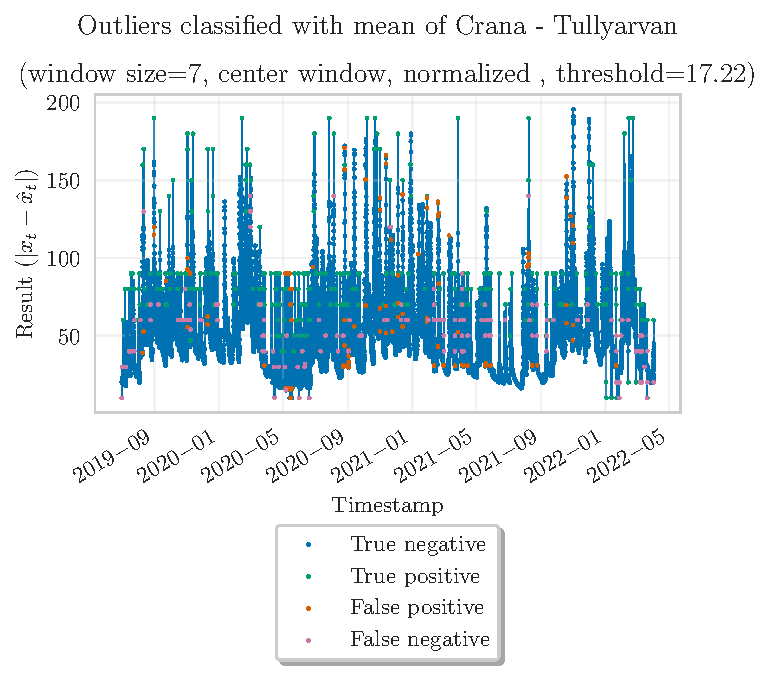
\includegraphics{plots/pdfs/39003-ie/od_mean_39003-ie_all.pdf}
    \caption{Best performance of outlier detection using mean (Crana - Tullyarvan)}
    \label{figure:od-mean-39003-ie}
\end{figure}

\subsubsection{Median}
\autoref{figure:od-median-2720050000-de} shows the best performing outlier detection using mean. The $F_1-score$ is about 0.91. % 0.9051094890510949
\begin{figure}[htp]
    \centering 
    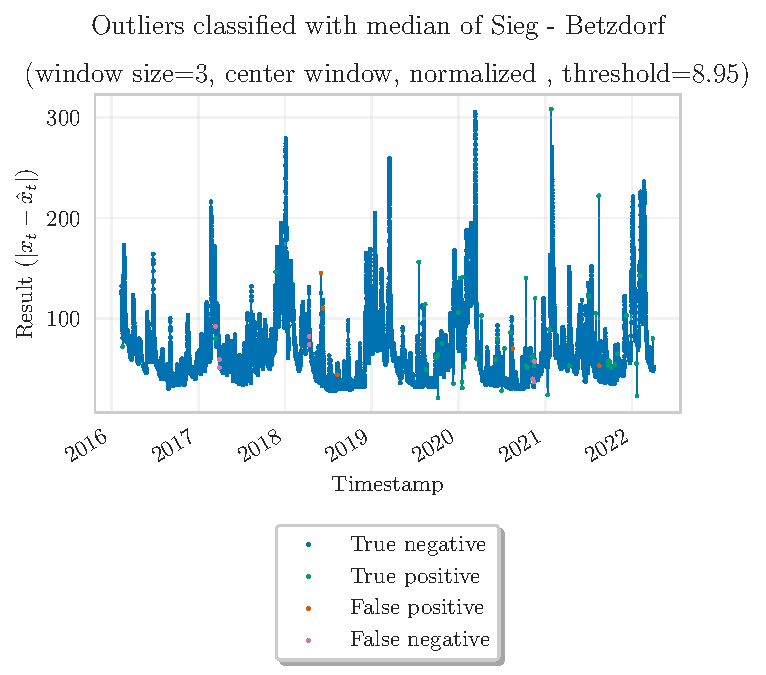
\includegraphics{plots/pdfs/2720050000-de/od_median_2720050000-de_all.pdf}
    \caption{Best performance of outlier detection using median (Sieg - Betzdorf)}
    \label{figure:od-median-2720050000-de}
\end{figure}
\subsubsection{MAD}
\autoref{figure:od-mad-42960105-de} shows the best performing outlier detection using mean. The $F_1-score$ is about 0.45. % 0.45454545454545453
\begin{figure}[htp]
    \centering 
    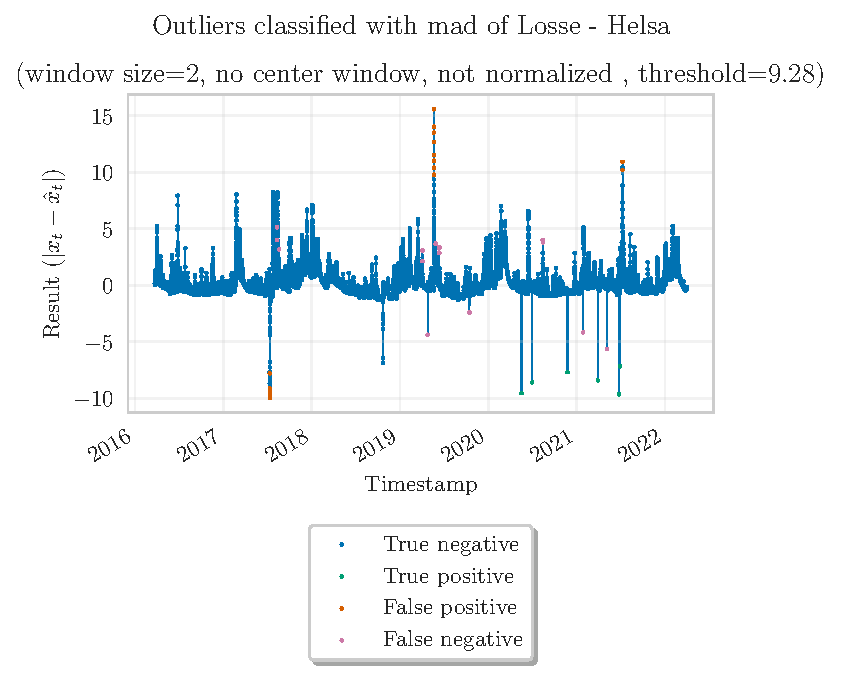
\includegraphics{plots/pdfs/42960105-de/od_mad_42960105-de_all.pdf}
    \caption{Best performance of outlier detection using mad (Losse - Helsa)}
    \label{figure:od-mad-42960105-de}
\end{figure}

\subsubsection{Z-score}
\autoref{figure:od-z-score-39003-ie} shows the best performing outlier detection using mean. The $F_1-score$ is about 0.68. % 0.6776677667766777
\begin{figure}[htp]
    \centering 
    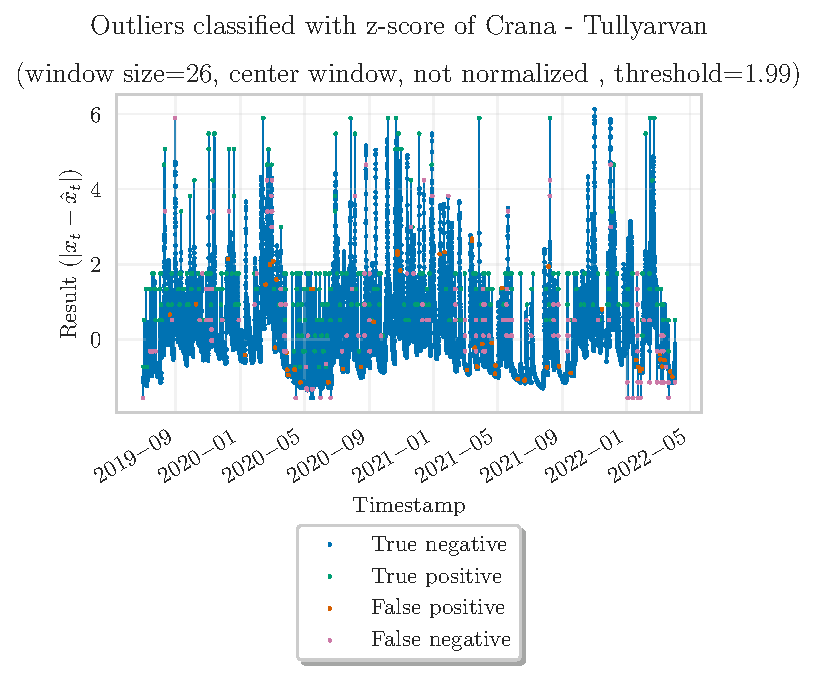
\includegraphics{plots/pdfs/39003-ie/od_z-score_39003-ie_all.pdf}
    \caption{Best performance of outlier detection using mad (Crana - Tullyarvan)}
    \label{figure:od-z-score-39003-ie}
\end{figure}

\subsubsection{MADN-z-score}
\autoref{figure:od-madn-z-score-36022-ie} shows the best performing outlier detection using mean. The $F_1-score$ is about 0.79. % 0.7892049598832969
\begin{figure}[htp]
    \centering 
    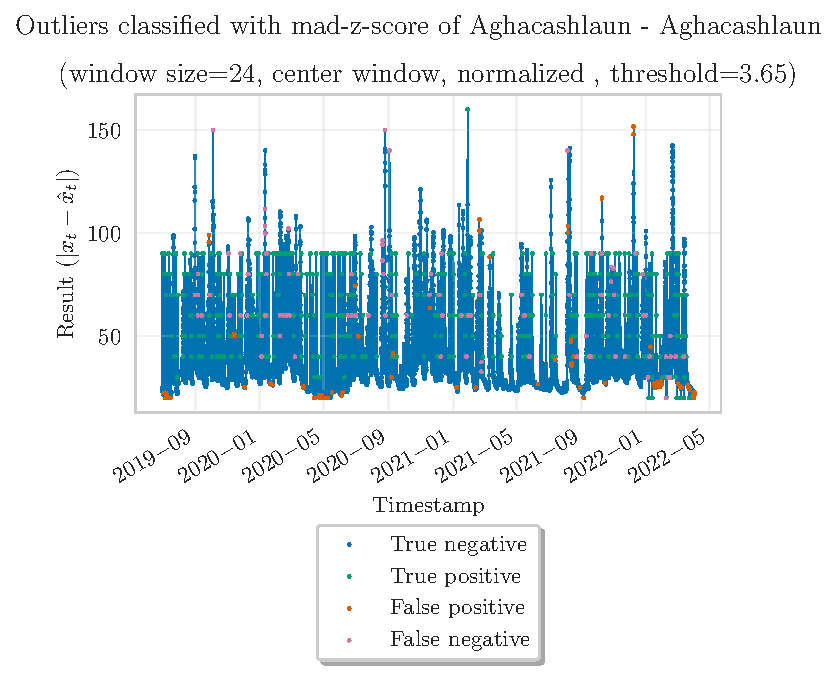
\includegraphics{plots/pdfs/36022-ie/od_mad-z-score_36022-ie_all.pdf}
    \caption{Best performance of outlier detection using \ac{MADN}-z-score (Aghacashlaun - Aghacashlaun)}
    \label{figure:od-madn-z-score-36022-ie}
\end{figure}

\subsection{Station 36022-ie}
\autoref{table:36022-ie-top-predictions-summary} shows the top three predictions per model for normalized and not normalized data. It clearly pictures, that methods using a centered moving window perform better. It is also interesting to see that the \ac{MADN} z-score and the regular z-score performed equally well regardless of the fact that the data is normalized or not. \todo{think of explanation for that.}
\todo{change mad-z-score to madn-z-score}
\begin{table}[htp]
\centering
\begin{tabular}{rllrlr}
\toprule
 window\_size &  center\_window &  normalized &  threshold &   model\_type &  f1\_score \\
\midrule
         5.0 &           True &       False &   7.622074 &       median &  0.812550 \\
         5.0 &           True &       False &   8.284281 &       median &  0.812348 \\
         5.0 &           True &       False &   7.953177 &       median &  0.811688 \\
        24.0 &           True &        True &   3.648829 & madn-z-score &  0.789205 \\
        24.0 &           True &       False &   3.648829 & madn-z-score &  0.789205 \\
        22.0 &           True &        True &   3.648829 & madn-z-score &  0.787572 \\
        22.0 &           True &       False &   3.648829 & madn-z-score &  0.787572 \\
        26.0 &           True &        True &   4.311037 & madn-z-score &  0.786415 \\
        26.0 &           True &       False &   4.311037 & madn-z-score &  0.786415 \\
         9.0 &           True &        True &   1.000000 &       median &  0.759430 \\
         7.0 &           True &        True &   1.000000 &       median &  0.750670 \\
         8.0 &           True &        True &   1.000000 &       median &  0.749358 \\
        24.0 &           True &       False &   1.993311 &      z-score &  0.626321 \\
        32.0 &           True &        True &   2.324415 &      z-score &  0.622718 \\
        32.0 &           True &       False &   2.324415 &      z-score &  0.621457 \\
        23.0 &           True &        True &   1.993311 &      z-score &  0.621359 \\
        27.0 &           True &        True &   2.324415 &      z-score &  0.620833 \\
        27.0 &           True &       False &   2.324415 &      z-score &  0.620833 \\
         9.0 &           True &       False &  16.892977 &         mean &  0.619647 \\
        10.0 &           True &       False &  18.879599 &         mean &  0.619173 \\
        10.0 &           True &       False &  19.210702 &         mean &  0.618538 \\
        11.0 &           True &        True &   1.331104 &         mean &  0.611993 \\
         9.0 &           True &        True &   1.331104 &         mean &  0.611418 \\
        10.0 &           True &        True &   1.331104 &         mean &  0.610659 \\
        24.0 &           True &        True &   1.993311 &          mad &  0.404255 \\
        26.0 &           True &        True &   1.993311 &          mad &  0.404000 \\
        28.0 &           True &        True &   1.993311 &          mad &  0.403183 \\
        22.0 &           True &       False &  66.889632 &          mad &  0.401679 \\
        22.0 &           True &       False &  67.220736 &          mad &  0.401126 \\
        22.0 &           True &       False &  67.551839 &          mad &  0.400856 \\
\bottomrule
\end{tabular}
\caption{Top predictions summary of Aghacashlaun - Aghacashlaun}
\label{table:36022-ie-top-predictions-summary}
\end{table}


\subsection{Station 2386-ch}
In \autoref{table:2386-ch-top-predictions-summary} the top three predictions per model for normalized and not not normalized data is shown. The outlier detection for this station has the worst performance among those tested. The result of this model is shown in \autoref{figure:od-result-example-2386-ch}. Every value above the threshold is classified as an outlier. Every value below the threshold is classified as a regular value.

\begin{figure}[htp]
    \centering 
    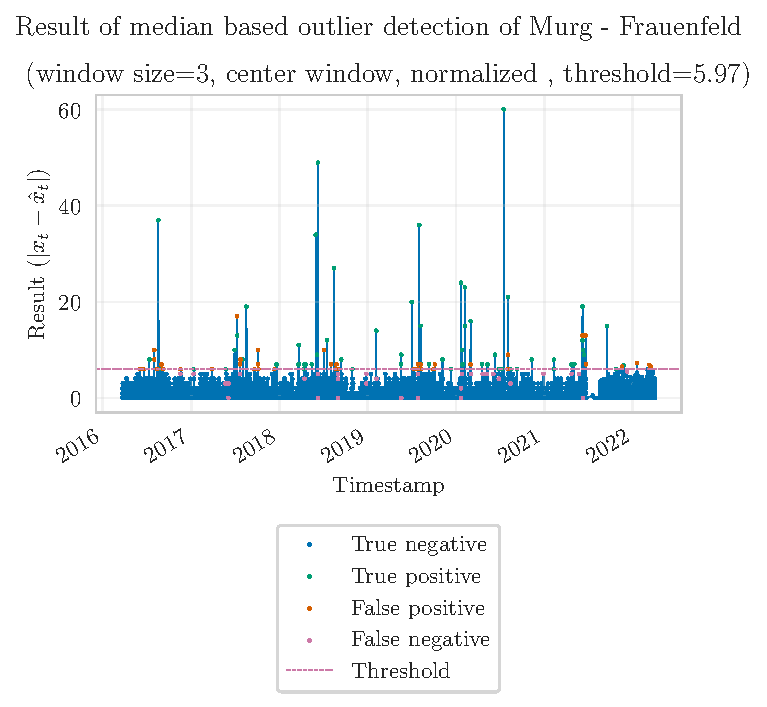
\includegraphics{plots/pdfs/2386-ch/od_result_median_2386-ch_all.pdf}
    \caption{Result of median based outlier detection Murg - Frauenfeld}
    \label{figure:od-result-example-2386-ch}
\end{figure}


\begin{table}[htp]
\centering
\begin{tabular}{rllrlr}
\toprule
 window\_size &  center\_window &  normalized &  threshold &  model\_type &  f1\_score \\
\midrule
         3.0 &           True &       False &   5.966555 &      median &  0.657895 \\
         3.0 &           True &       False &   5.635452 &      median &  0.649351 \\
         3.0 &           True &       False &   6.628763 &      median &  0.639175 \\
         3.0 &           True &       False &   4.642140 &        mean &  0.447917 \\
         3.0 &           True &       False &   4.973244 &        mean &  0.443804 \\
         3.0 &           True &       False &   5.304348 &        mean &  0.429907 \\
        50.0 &           True &        True &   3.979933 &     z-score &  0.327273 \\
        50.0 &           True &       False &   3.979933 &     z-score &  0.327273 \\
        49.0 &           True &        True &   3.648829 &     z-score &  0.306931 \\
        49.0 &           True &       False &   3.648829 &     z-score &  0.306931 \\
        48.0 &           True &       False &   3.648829 &     z-score &  0.305419 \\
        50.0 &           True &        True &   3.648829 &     z-score &  0.303922 \\
        47.0 &           True &        True &   1.000000 &      median &  0.120690 \\
        42.0 &          False &        True &  11.926421 &      median &  0.120690 \\
        42.0 &          False &        True &   8.946488 &      median &  0.120690 \\
        49.0 &          False &        True &  24.177258 &        mean &  0.120690 \\
        34.0 &           True &        True &   9.277592 &        mean &  0.120690 \\
        34.0 &           True &        True &   6.959866 &        mean &  0.120690 \\
         NaN &           True &        True &  61.591973 & mad-z-score &  0.120690 \\
         NaN &          False &        True &  97.351171 & mad-z-score &  0.120690 \\
         NaN &          False &        True &  98.013378 & mad-z-score &  0.120690 \\
         NaN &           True &       False &  61.591973 & mad-z-score &  0.120690 \\
         NaN &          False &       False &  97.351171 & mad-z-score &  0.120690 \\
         NaN &          False &       False &  98.013378 & mad-z-score &  0.120690 \\
         7.0 &           True &        True &   1.000000 &         mad &  0.120690 \\
        11.0 &           True &        True &   1.993311 &         mad &  0.120690 \\
        34.0 &          False &        True &  24.839465 &         mad &  0.120690 \\
         7.0 &           True &       False &   1.000000 &         mad &  0.004301 \\
        27.0 &           True &       False &   4.973244 &         mad &  0.004301 \\
        27.0 &           True &       False &   5.635452 &         mad &  0.004301 \\
\bottomrule
\end{tabular}
\caption{Top predictions summary of Murg - Frauenfeld}
\label{table:2386-ch-top-predictions-summary}
\end{table}


\subsection{Station 2720050000-de}
In \autoref{table:2720050000-de-top-predictions-summary} the top three predictions per model for normalized and not not normalized data is shown. With an $F_1-score$ of 0.905109 this station had the best performance. The result of this model is shown in \autoref{figure:od-result-example-202720050000-de}. Every value above the threshold is classified as an outlier. Between 2018 and 2019 an example of a \ac{FP} can be seen (the orange values above the threshold).

\begin{figure}[htp]
    \centering 
    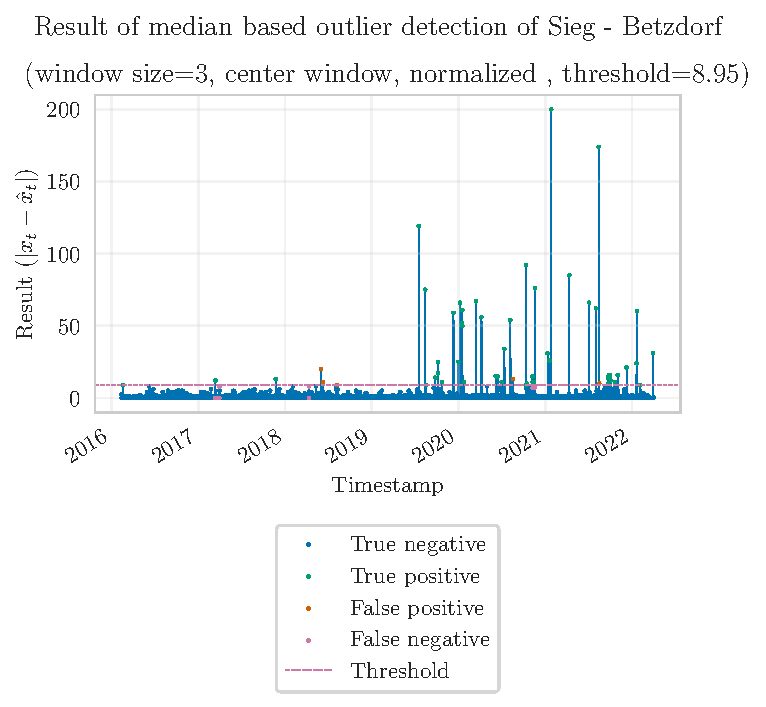
\includegraphics{plots/pdfs/2720050000-de/od_result_median_2720050000-de_all.pdf}
    \caption{Result of median based outlier detection Sieg - Betzdorf}
    \label{figure:od-result-example-202720050000-de}
\end{figure}

\begin{table}[htp]
\centering
\begin{tabular}{rllrlr}
\toprule
 window\_size &  center\_window &  normalized &  threshold &   model\_type &  f1\_score \\
\midrule
         3.0 &           True &       False &   8.284281 &       median &  0.905109 \\
         3.0 &           True &       False &   8.615385 &       median &  0.905109 \\
         3.0 &           True &       False &   8.946488 &       median &  0.905109 \\
        29.0 &           True &       False &   3.648829 &      z-score &  0.545455 \\
        23.0 &           True &       False &   3.317726 &      z-score &  0.545455 \\
        27.0 &           True &       False &   3.648829 &      z-score &  0.542373 \\
        22.0 &           True &        True &   3.317726 &      z-score &  0.533333 \\
        28.0 &           True &        True &   3.648829 &      z-score &  0.533333 \\
        20.0 &           True &        True &   3.317726 &      z-score &  0.516667 \\
         3.0 &           True &       False &   7.290970 &         mean &  0.510288 \\
         3.0 &           True &       False &   6.959866 &         mean &  0.510121 \\
         3.0 &           True &       False &   6.628763 &         mean &  0.503937 \\
         NaN &          False &        True &  10.602007 & madn-z-score &  0.133333 \\
         NaN &           True &        True &  10.602007 & madn-z-score &  0.133333 \\
         NaN &          False &       False &  10.602007 & madn-z-score &  0.133333 \\
         NaN &           True &       False &  10.602007 & madn-z-score &  0.133333 \\
         NaN &          False &        True &  10.270903 & madn-z-score &  0.119048 \\
         NaN &          False &       False &  10.270903 & madn-z-score &  0.119048 \\
        47.0 &           True &        True &   1.000000 &       median &  0.108108 \\
        29.0 &          False &        True &   1.000000 &       median &  0.108108 \\
        50.0 &          False &        True &   2.324415 &       median &  0.108108 \\
         NaN &          False &        True &   1.662207 &         mean &  0.108108 \\
         NaN &           True &        True &   1.662207 &         mean &  0.108108 \\
         NaN &           True &        True &   1.000000 &         mean &  0.108108 \\
         7.0 &           True &        True &   1.000000 &          mad &  0.108108 \\
        31.0 &           True &        True &   1.000000 &          mad &  0.108108 \\
        25.0 &          False &        True &   2.324415 &          mad &  0.108108 \\
        49.0 &           True &       False & 100.000000 &          mad &  0.006390 \\
        50.0 &           True &       False & 100.000000 &          mad &  0.006379 \\
        47.0 &           True &       False & 100.000000 &          mad &  0.006360 \\
\bottomrule
\end{tabular}
\caption{Top predictions summary of Sieg - Betzdorf}
\label{table:2720050000-de-top-predictions-summary}
\end{table}


\subsection{Station 42960105-de}
In \autoref{table:42960105-de-top-predictions-summary} the top three predictions per model for normalized and not not normalized data is shown.
\begin{table}[htp]
\footnotesize
\centering
\begin{tabular}{rllrlr}
\toprule
 window\_size &  center\_window &  normalized &  threshold &   model\_type &  f1\_score \\
\midrule
         6.0 &           True &        True &   2.655518 &       median &  0.731707 \\
         4.0 &           True &       False &  25.170569 &       median &  0.731707 \\
         4.0 &           True &       False &  26.494983 &       median &  0.731707 \\
         4.0 &           True &       False &  26.163880 &       median &  0.731707 \\
         3.0 &           True &        True &   1.000000 &       median &  0.720000 \\
         4.0 &           True &        True &   2.324415 &       median &  0.714286 \\
        19.0 &           True &        True &   5.966555 &         mean &  0.571429 \\
        17.0 &           True &        True &   5.635452 &         mean &  0.571429 \\
        15.0 &           True &        True &   5.304348 &         mean &  0.571429 \\
        15.0 &           True &       False &  62.585284 &         mean &  0.571429 \\
        16.0 &           True &       False &  62.585284 &         mean &  0.571429 \\
        16.0 &           True &       False &  59.605351 &         mean &  0.571429 \\
         2.0 &          False &        True &   9.277592 &          mad &  0.454545 \\
         2.0 &           True &        True &   9.277592 &          mad &  0.454545 \\
         2.0 &          False &        True &   9.939799 &          mad &  0.439024 \\
         NaN &           True &        True &  18.879599 &      z-score &  0.275862 \\
         NaN &           True &        True &  17.555184 &      z-score &  0.275862 \\
         NaN &          False &        True &  16.892977 &      z-score &  0.275862 \\
         NaN &          False &       False &  19.541806 &      z-score &  0.275862 \\
         NaN &          False &       False &  16.561873 &      z-score &  0.275862 \\
         NaN &          False &       False &  15.899666 &      z-score &  0.275862 \\
         NaN &          False &        True &  30.137124 & madn-z-score &  0.275862 \\
         NaN &          False &        True &  32.785953 & madn-z-score &  0.275862 \\
         NaN &          False &        True &  35.103679 & madn-z-score &  0.275862 \\
         NaN &          False &       False &  30.137124 & madn-z-score &  0.275862 \\
         NaN &          False &       False &  32.785953 & madn-z-score &  0.275862 \\
         NaN &          False &       False &  35.103679 & madn-z-score &  0.275862 \\
         NaN &           True &       False & 100.000000 &          mad &  0.005068 \\
         NaN &          False &       False & 100.000000 &          mad &  0.005068 \\
         NaN &           True &       False &  99.668896 &          mad &  0.004548 \\
\bottomrule
\end{tabular}
\caption{Top predictions summary of Losse - Helsa}
\label{table:42960105-de-top-predictions-summary}
\end{table}


\subsection{Station 39003-ie}
In \autoref{table:39003-ie-top-predictions-summary} the top three predictions per model for normalized and not not normalized data is shown.
\begin{table}[htp]
\footnotesize
\centering
\begin{tabular}{rllrlr}
\toprule
 window\_size &  center\_window &  normalized &  threshold &   model\_type &  f1\_score \\
\midrule
         5.0 &           True &       False &   8.615385 &       median &  0.859035 \\
         5.0 &           True &       False &   9.277592 &       median &  0.858500 \\
         5.0 &           True &       False &   8.946488 &       median &  0.857685 \\
        34.0 &           True &        True &   3.648829 & madn-z-score &  0.736842 \\
        34.0 &           True &       False &   3.648829 & madn-z-score &  0.736842 \\
        34.0 &           True &        True &   4.311037 & madn-z-score &  0.733962 \\
        34.0 &           True &       False &   4.311037 & madn-z-score &  0.733962 \\
        32.0 &           True &        True &   4.642140 & madn-z-score &  0.731707 \\
        32.0 &           True &       False &   4.642140 & madn-z-score &  0.731707 \\
        11.0 &           True &        True &   1.000000 &       median &  0.723699 \\
        10.0 &           True &        True &   1.000000 &       median &  0.723059 \\
         9.0 &           True &        True &   1.000000 &       median &  0.720189 \\
         7.0 &           True &       False &  17.224080 &         mean &  0.684211 \\
         7.0 &           True &       False &  16.230769 &         mean &  0.683398 \\
         7.0 &           True &       False &  16.892977 &         mean &  0.683267 \\
        26.0 &           True &        True &   1.993311 &      z-score &  0.677668 \\
        26.0 &           True &       False &   1.993311 &      z-score &  0.677668 \\
        27.0 &           True &        True &   1.993311 &      z-score &  0.672489 \\
        27.0 &           True &       False &   1.993311 &      z-score &  0.672489 \\
        25.0 &           True &        True &   1.993311 &      z-score &  0.669633 \\
        25.0 &           True &       False &   1.993311 &      z-score &  0.669633 \\
         8.0 &           True &        True &   1.000000 &         mean &  0.643868 \\
         9.0 &           True &        True &   1.000000 &         mean &  0.636678 \\
        10.0 &           True &        True &   1.000000 &         mean &  0.633596 \\
        36.0 &           True &       False &  85.431438 &          mad &  0.180556 \\
        34.0 &           True &       False &  85.431438 &          mad &  0.180149 \\
        36.0 &           True &       False &  85.100334 &          mad &  0.179840 \\
        30.0 &           True &        True &   1.662207 &          mad &  0.173418 \\
        14.0 &          False &        True &   1.662207 &          mad &  0.173355 \\
        29.0 &           True &        True &   1.662207 &          mad &  0.173149 \\
\bottomrule
\end{tabular}
\caption{Top predictions summary of Crana - Tullyarvan}
\label{table:39003-ie-top-predictions-summary}
\end{table}


% Compare detection methods from the previous section.
% \todo{write}


\chapter{Conclusion}
This bachelor thesis provides an overview of the topic anomaly detection, especially on outlier detection for time series data. It provides a description for key features of data quality, and introduces the topic of data cleaning and data cleansing. Furthermore this paper provides general overview of outlier detection approaches. After a theoretical overview of different outlier detection approaches they are tested on water level data from different rivers.
\par
% There are countless methods to detect anomalies in data. There is not a go-to approach that suits all needs. It is required to assess different approaches for different applications, in order to get the best result. This paper should provide an overview of approaches to detect outliers / anomalies. It depends on the use case which method to detect outliers has the highest success rate.  
The overall bes performance, across different water level measurement stations, was achieved by using the median threshold based outlier detection method with a centered window with the size of three and a threshold of about 6.6. The median threshold based outlier detection also delivered the hightest $F_1-score\;(0.905)$. Using the mean to calculate $\hat{x}_t$ is not recommended since the mean is not robust against outliers. Using the \ac{MAD} with the threshold based outlier detection resulted in the lowest $F_1-score$, with the best score only being about 0.45. The second best result was achieved by using the modified z-score described in \autoref{section:outlier-detection-modified-z-score}. For the stations tested the approach using the median delivered the best performances. However this does not mean, that this will be true for all stations. It has to be assessed for each station individually which model is able to detect best. Furthermore it depends on the use case if higher precision or recall is required. Depending on that, $\beta$ for the $F_{\beta}-score$ needs to be chosen accordingly. For the tests the $F_1-score$ was used since precision and recall are equally important. In addition preprocessing the data by setting upper and lower boundaries and removing datapoints which exceed those limits, did not improve the performance of the models, on the contrary the performance was worse. Because the extreme outliers were mostly detected anyways, thus fewer outliers were detected when setting upper and lower limits, which resulted in a lower performance.

\change{Ich schlage hier vor auch einen Teil der quanitativen Analyse zusammenzufassen. Dabei sollten die Methoden und die Ergebnisse kurz skizziert werden. Vielleicht lassen sich auch Entscheidungen ableiten wann welche Methode besser greift.}
% \todo{Change this! Currently copied from the paper.}
% \section{Advantages and Disadvantages of used Outlier Detection Methods}
% \todo{write}
\chapter{Future Work}
Chapter about which additional approaches could be tested:
\begin{itemize}
    \item setting a maximum gradient for both directions (one for rising and falling values) for each measurement station.
    \item \acp{ANN} with \ac{LSTM} or \ac{GRU} maybe also autoencoder architecture
    \item Prediction vs classification \ac{ANN}
    \item 1.5 times the \ac{IQR}
\end{itemize} 
\todo{Should I also include this or is this not common for a bachelor thesis? -> YES}
\change{Die Methode wollte ich auch vorschlagen, aber der Umfang ist so schon gross genug.}
\newpage
\bibliographystyle{IEEEtran}

\bibliography{bachelor_thesis}


% List of figures
\newpage
\listoffigures


% List of tables
\newpage
\listoftables
\clearpage

% List of source codes
\renewcommand\listoflistingscaption{List of source codes}
\listoflistings
\clearpage

% List of Algorithms
%\listofalgorithms
%\clearpage

% List of Abbreviations
\phantomsection
\addcontentsline{toc}{chapter}{List of Abbreviations}
\chapter*{List of Abbreviations}
\begin{acronym}%[XXXXX]
	\acro{IoT}[IoT]{Internet of Things}
	\acro{CSV}[CSV]{Comma Separated Values }
	\acro{JSON}[JSON]{Java Script Object Notation}
	\acro{MAD}[MAD]{Mean Absolute Deviation}
	\acro{LSTM}[LSTM]{Long Short-Term Memory}
	\acro{GRU}[GRU]{Gated Recurrent Unit}
	\acro{ARIMA}[ARIMA]{AutoRegressive Integrated Moving Average}
	\acro{GP}[GP]{Gaussian Process}
	\acro{HMAC}[HMAC]{Keyed-Hashing for Message Authentication}
\end{acronym}


\end{document}